\documentclass[10pt,usenames,xcolor=dvipsnames]{report}

%%% Packages %%%

\usepackage{amsmath, bm}
\usepackage[backend=biber, alldates=iso]{biblatex}
  \addbibresource{bibliography.bib}
\usepackage{blindtext}
\usepackage{enumitem} % itemize alignment
\usepackage{caption}
\usepackage{float}
\usepackage[T1]{fontenc}
\usepackage{fontspec}
  \setmainfont[
    Path = ./fonts/,
    BoldFont = main-bold,
    BoldItalicFont = main-bold-italic,
    ItalicFont = main-italic,
    Extension = .ttf
  ]{main-regular.ttf}
  \setmonofont[
    Path = ./fonts/,
    BoldFont = mono-bold,
    BoldItalicFont = mono-bold-italic,
    ItalicFont = mono-italic,
    Extension = .ttf
  ]{mono-regular.ttf}

% Geometry setup and styling reside in a separate file
\newcommand{\paperWidth}{210 mm}      % page width
\newcommand{\paperHeight}{297 mm}     % page height
\newcommand{\marginLeft}{15 mm}       % margin between text and left end of page
\newcommand{\marginRight}{15 mm}      % margin between text and right end of page
\newcommand{\marginBottom}{15 mm}     % margin between footer line and bottom end of page
\newcommand{\textMarginBottom}{25 mm} % margin between text and bottom end of page
\newcommand{\columnSep}{10 mm}        % margin between columns for 2-col layout
\newcommand{\logoWidth}{30 mm}        % Width of JS-Soft logo in page footer

% Load geometry package and define \left and \right, which otherwise is
% impossible to directly via \setlength.

\usepackage[
  paperwidth=\paperWidth,   % page width
  paperheight=\paperHeight, % page heigth
  left=\marginLeft,         % margin between text and right end of page
  right=\marginRight,       % margin between text and right end of page
  bottom=\textMarginBottom, % margin between text and right end of page
  columnsep=\columnSep      % margin between columns for 2-col layout
    ]{geometry}

%%%%%%%%%%%%%%%%%%%%%%%%%%%
%%%%% Spacing & Indentation
%%%%%%%%%%%%%%%%%%%%%%%%%%%

% Increase linespread a bit (eyeballed)

\linespread{1.2}

% Set paragraph spacing to 6pt

\setlength{\parskip}{6pt}

% Remove paragraph indentation

\setlength{\parindent}{0pt}

\todo{Seitenlayout für Druck anpassen}


\usepackage{graphicx}
  \graphicspath{{./assets/}}
\usepackage[hidelinks,linktocpage=true,colorlinks=true,citecolor=red]{hyperref}
\usepackage[outputdir=build]{minted}
\usepackage{nicematrix} % Better matrices
\usepackage{todo} % Add todos and create an index of all todos.
\usepackage{svg}
\usepackage{titlesec}
\usepackage{tikz}
  \usetikzlibrary{backgrounds,calc,fit,positioning,shadows.blur,tikzmark,arrows.meta,shapes,matrix}
\usepackage{tocbibind}
  \settocbibname{References}
\usepackage{xcolor}

% Miscellaneous

\renewcommand{\contentsname}{Table of Contents} % Set display name of ToC

\definecolor{gray75}{gray}{0.75}
\definecolor{monokaibg}{HTML}{272822}
\definecolor{dodgerblue4}{HTML}{31475E}
\definecolor{mygreen}{rgb}{0.0, 0.5, 0.0}

\titleformat{\chapter}[hang]{\Huge\bfseries}{\thechapter\hspace{20pt}\textcolor{gray75}{\rule[-4.0mm]{0.50mm}{12.00mm}}\hspace{20pt}}{0pt}{\Huge\bfseries}
\titlespacing*{\chapter}{0pt}{-20pt}{40pt}

% Load custom commands

%
% Definition of custom commands
%
\usepackage{xparse}


%%
%% Define commands for formatting C3srMatrix data members correctly
%%
\NewDocumentCommand{\DataMember}{ m o }
  {
  \ifmmode
     \text{#1}\IfNoValueF{#2}{[#2]}
   \else
     #1\IfNoValueF{#2}{[#2]}
   \fi
  }

\NewDocumentCommand{\V}{o}
  {\DataMember{V}[#1]}
\NewDocumentCommand{\VS}{o}
  {\DataMember{VS}[#1]}
\NewDocumentCommand{\J}{o}
  {\DataMember{J}[#1]}
\NewDocumentCommand{\JS}{o}
  {\DataMember{JS}[#1]}
\NewDocumentCommand{\JP}{o}
  {\DataMember{JP}[#1]}
\NewDocumentCommand{\RS}{o}
  {\DataMember{RS}[#1]}
\NewDocumentCommand{\RP}{o}
  {\DataMember{RP}[#1]}
\NewDocumentCommand{\CI}{o}
  {\DataMember{CI}[#1]}

% keyword
\NewDocumentCommand\keyword{m}{\textbf{\emph{#1}}}

% toccaption - Repeat TOF caption in bold-face as first sentence of the figure's caption.
\NewDocumentCommand\toccaption{m m}{\caption[#1]{\small\textbf{#1} {#2}}}


% Begin document

\begin{document}

  % Titlepage

  \begin{titlepage}
\begin{tikzpicture}[
  remember picture,
  overlay
    ]
  \node[anchor=center,
        font=\Huge,
        align=center] (TITLE)
    at ($(current page.north west)+(0.5\paperwidth, -5)$)
    {A High-Performance Matrix Storage\\Format for Sparse Banded Matrices\\Derived from Structured Grids};
  \node[below=10cm of TITLE,
        align=center,
        font=\Large] (DESCR)
    {\textbf{Master Thesis} in \textbf{Computer Engineering}\\submitted to the\\\textbf{Department of Physics and
    Astronomy, University of Heidelberg}\\by\\\textbf{Stanislaw Hüll}\\born November $25^{\text{th}}$, $1990$ in
     Rostov-on-Don};
  \node[below=2cm of DESCR, align=center] (DESCR2)
    {This Master thesis has been carried out at the \textbf{Institute of Computer Engineering (ZITI)}\\ at the
    \textbf{University of Heidelberg} under the supervision of Prof. Dr. Robert Strzodka.\\
    \newline \\
    First Corrector: Prof. Dr. Robert Strzodka \\
    Second Corrector: Prof. Dr. Guido Kanschat};
\end{tikzpicture}
\end{titlepage}


  % Abstract

  \def\abstractWidth{14cm}

\NewDocumentCommand{\abstrTitleStyle}{ m }{\center{\Large\textbf{#1}}\\\vspace{5mm}}

\begin{tikzpicture}[
  remember picture,
  overlay
    ]
  \node[anchor=north,
        font=\normalsize,
        align=justify,
        text width=\abstractWidth] (ABSTRACT-EN)
    at ($(current page.north west)+(0.5\paperwidth, -5)$)
    {\abstrTitleStyle{Abstract}

      Many domains of the physical sciences such as computational fluid dynamics and electrodynamics use simulations
      based on known governing laws to gather insights into a system's transient or static behavior. Where geometries
      are regular structured grids are utilized in the modelling process for their good performance due to the inherent
      structural simplicity. The solution procedure involves matrix-vector multiplications on the sparse system matrix
      which are implemented using different general purpose sparse matrix storage formats, such as the compressed sparse
      row format (CSR). This thesis introduces the threefold compressed sparse row matrix storage format (C3SR) designed
      for compact storage and fast arithmetic of sparse banded matrices derived from structured grids. The storage
      format, its compression method and arithmetic schemes are presented and evaluated in a series of tests and
      benchmarks. Compression is found to perform very well and to be stable with respect to perturbations of a grid's
      regularity. Arithmetic performance is evaluated on three systems with varying, possibly promising results which
      suggest further inquiry. Follow-up work is suggested in the outlook.};

  \node[below=1cm of ABSTRACT-EN,
        align=justify,
        font=\normalsize,
        text width=\abstractWidth] (ABSTRACT-DE)
    {\abstrTitleStyle{Zusammenfassung}

    Viele Teilbereiche der Naturwissenschaft verwenden ihr Verständnis über die herrschenden Gesetze eines Systems um
    mittels Simulationen Einblicke in das Verhalten des Systems zu gewinnen. Probleme, deren Domäne aus regulären
    Strukturen aufgebaut ist werden häufig auf Grundlage von strukturierten Gittern modelliert um deren geringere
    Komplexität zur Beschleunigung der Simulation zu verwenden. Lösungsverfahren erzeugen eine dünnbesetze, aus
    digonalen Bändern aufgebaue Systemmatrix, welche für eine Vielzahl von Matrix-Vektor Multliplikationen benötigt
    wird, die mittels üblicher Speicherformate für dünnbesetze Matrizen implementiert wird. Diese Arbeit stellt eine
    Abwandlung des gebräuchlichen Compressed Sparse Row (CSR) Formats vor, das Threefold Compressed Sparse Row (C3SR)
    Format, welches für kompaktes Speichern und performante Arithmetik von dünnbesetzen Matrizen, welche von
    strukturierten Gittern abgeleitet wurden, entworfen wurde. Das Format, das Kompressionsmethode und die
    Multiplikationsschemata werden vorgestellt und auf Leistung untersucht. Das Kompressionsverfahren erzielt auch bei
    Störung der Regularität der Gitter sehr gute Ergebnisse. Die Matrix-Vektor Multiplikation wird auf 3 Systemen
    getestet und kann unterschiedliche, zum Teil aber erfolgsversprechende Ergebnisse aufweisen, welche weitere
    Analyse und Untersuchungen nahelegen. Vorschläge dafür sind im abschließenden Kapitel gelistet.
    };
\end{tikzpicture}

\newpage


  % Table of Contents

  \tableofcontents
  \listoffigures

%  \part{Threefold Compressed Sparse Row Matrix Storage Format}

    \chapter{Introduction}

  This section introduces two notions fundamental to the ideas developed in this report, the general purpose
  \keyword{compressed sparse row} matrix storage format (CSR) and, secondly, \keyword{sparse banded matrices} as well as
  their usage in the natural sciences and their particular structure.

  \section{Compressed Sparse Row Matrix Storage Format}

    The compressed sparse row (CSR) format is a widely used storage format for sparse matrices. Unlike other popular
    sparse matrix storage formats such as the diagonal storage format (DIA), the CSR format is not tailored to any
    special type of matrix but is a general purpose storage format that makes no assumptions about the matrix's shape or
    its distribution of non-zeros. The CSR format can be considered an improvement to the naive coordinate format (COO)
    in that each non-zero's row index is no longer explicitly stored \cite{Bell2011}.

    The CSR format consists of three dense arrays. The values array (V) stores the numerical value for each non-zero
    entry in the matrix while the associated column index is stored in the column-index array (CI). A third array, the
    row-pointer array (RP), encodes the beginning of each row's section within the values and column-index arrays, i.e.
    it stores the offset of each row's first non-zero element into the two arrays. By convention, the row-pointer array
    usually also contains an additional element denoting the total number of non-zero elements in the matrix. An example
    for the CSR format is given in Figure \ref{fig:csr_example}.

    \begin{figure}[ht]
      \centering
      \begin{minipage}{0.4\textwidth}
        \centering
        $$
        \begin{pmatrix}
          \color{red}{\bm{3}} &                     0 &  \color{red}{\bm{4}} &                    0 \\
                            0 & \color{green}{\bm{1}} &                    0 &                    0 \\
                            0 &                     0 & \color{blue}{\bm{7}} & \color{blue}{\bm{8}} \\
        \end{pmatrix}
        $$
      \end{minipage}
      \begin{minipage}{0.4\textwidth}
        \centering
        $$
        \begin{matrix}
          \text{Values}  & : & \color{red}{3} &   \color{red}{4} & \color{green}{1} & \color{blue}{7} & \color{blue}{8} \\
          \text{Column-Indices} & : & \color{red}{0} &   \color{red}{2} & \color{green}{1} & \color{blue}{2} & \color{blue}{3} \\
          \text{Row-Pointers} & : & \color{red}{0} & \color{green}{2} &  \color{blue}{3} &               5 &                 \\
        \end{matrix}
        $$
      \end{minipage}
      \caption[Exemplary matrix with corresponding CSR representation.]{\textbf{Exemplary matrix with corresponding CSR representation.} The array elements are color-coded in red for the first row, green for the second row and blue for the third row.}
      \label{fig:csr_example}
    \end{figure}

    Thus, as previously mentioned, the CSR format optimizes the storage requirements of general sparse matrices with
    respect to the naive coordinate format (COO) shrinking the size of the third array from one entry per non-zero
    element to a single entry per row irrespective of the row's number of non-zeros. Furthermore, the existing
    literature, in part, utilizes a different nomenclature referring to the arrays as A (values array), JA (column-index
    array) and IA (row-pointer array), respectively \cite{sparskit}.

    The CSR format's salient feature is the contiguousness of the rows' non-zero elements' values and column indices
    making it particularly well suited for matrix-vector-multiplication utilizing a conventional row-by-column
    computation scheme due to ideal data locality for the values and column arrays. Aside of this characteristic storing
    the non-zero elements row-by-row as opposed to column-by-column is a choice and thus exist numerical libraries and
    toolkits such as the Eigen C++ library \cite{eigen:website} or the Harwell-Boeing sparse matrix collection
    \cite{harwell-boeing} which utilize the CSR format's conjugate, the compressed sparse column format (CSC), as their
    default means of storing sparse matrices.

    The CSR format serves as a starting point for the C3SR sparse matrix storage format for sparse banded matrices which
    is the focal point of this work.

    \Todo{CSR expandieren}

  \section{Sparse Banded Matrices Derived from Structured Grids} \label{sec:structured-grid-matrices}

    Structured grid computations are ubiquitously used for physical simulations in scientific fields such as, for
    example, computational fluid dynamics, electrodynamics and astrophysics. Generally, a system of partial differential
    equations is solved by discretization and linearization of the problem which involves generating a grid
    corresponding to the physical domain in question. A structured grid refers to a mesh whose nodes are uniquely
    identified by a tuple of coordinates and v.v., such as $(i, j, k)$ for three dimensions (Figure
    \ref{fig:structured_grid_example}). Such meshes are sometimes referred to as \emph{logically rectangular}.

    \begin{figure}[ht]
        \centering
        \vspace{0.5cm}
        \begin{minipage}{0.4\textwidth}
          \centering
          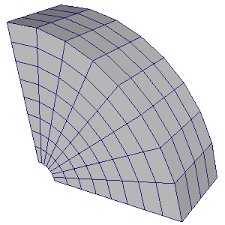
\includegraphics[width=0.9\textwidth]{fig/structured_grid_example.png} % second figure itself
          \caption[Curvi-linear grid over a physically complex domain.]{\textbf{Curvi-linear grid over a physically complex domain.} The grid nodes are logically rectangular despite the non-rectangular physical domain and thus comprise a structured grid. Source: \cite{daad:website}}
          \label{fig:structured_grid_example}
        \end{minipage}\hfill
        \begin{minipage}{0.5\textwidth}
          \centering
          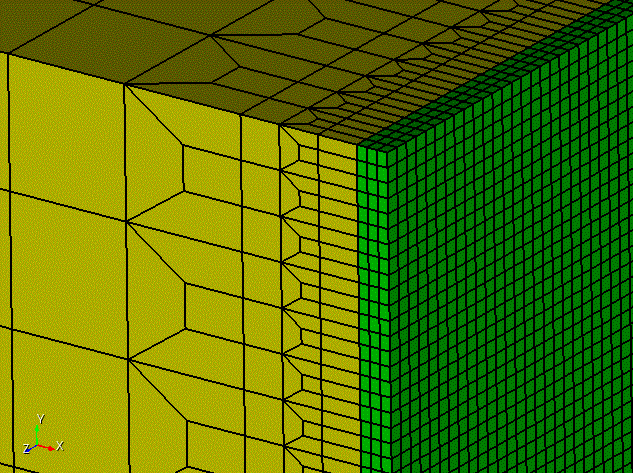
\includegraphics[width=0.9\textwidth]{fig/refined_structured_grid.png} % second figure itself
          \caption[Heterogeneous mesh with structured regions.]{\textbf{Heterogeneous mesh with structured regions.} Outer side (green) and interior volume are fully structured and are connected via an unstructured mesh region. Given proper indexing of grid nodes the resulting sparse matrix will exhibit regularity in the sections pertaining to the structured mesh region. Source: \cite{cubit-mesh-refinement:website}}
          \label{fig:refined_structured_grid}
        \end{minipage}
    \end{figure}

    In contrast to unstructured grids the regularity inherent to structured grids allows for very efficient numerical
    treatment, such that even in cases where sufficiently complex geometries prohibit the decomposition of the target
    domain into a single overarching structured grid the domain is often tesselated into an unstructured configuration,
    with the tiles being filled by independent structured grids \cite{Badcock2000}(Figure
    \ref{fig:refined_structured_grid}).

    \begin{figure}
        \centering
        \begin{minipage}{0.45\textwidth}
          \centering
          \begin{tikzpicture}[scale=0.65]%[every node/.style={minimum size=1cm},on grid]
\newcommand*{\height}{5}
\newcommand*{\width}{5}
\begin{scope}[every node/.append style={yslant=-0.5},yslant=-0.5]
  \shade[right color=gray!10, left color=black!50] (0,0) rectangle +(\width,\height);

  \foreach \x in {1,...,\width}
    \foreach \y in {1,...,\height}
    {
        \node at (-0.5 + \x, -0.5 + \y) {\pgfmathtruncatemacro\result{21-5*(\x-1)+25*(\y-1)}$\result$};
    }
  \draw (0,0) grid (\height,\width);
\end{scope}
\begin{scope}[every node/.append style={yslant=0.5},yslant=0.5]
  \shade[right color=gray!70,left color=gray!10] (\width,-\height) rectangle +(\height,\width);
    \foreach \x in {1,...,\width}
    \foreach \y in {1,...,\height}
    {
        \node at (\width - 0.5 + \x, -\height + -0.5 + \y) {\pgfmathtruncatemacro\result{1 + 1*(\x-1)+25*(\y-1)}$\result$};
    }

  \draw (\width,-\height) grid (2*\width,0);
\end{scope}
\begin{scope}[every node/.append style={
    yslant=0.5,xslant=-1},yslant=0.5,xslant=-1
  ]
  \shade[bottom color=gray!10, top color=black!80] (2*\width,\height) rectangle +(-\width,-\height);

    \foreach \x in {1,...,\width}
    \foreach \y in {1,...,\height}
    {
        \node at (\width - 0.5 + \x, -0.5 + \y) {\pgfmathtruncatemacro\result{101 + 1*(\x-1)+5*(\y-1)}$\result$};
    }

  \draw (\width,0) grid (2*\width,\height);
\end{scope}
\end{tikzpicture}

        \end{minipage}\hfill
        \begin{minipage}{0.45\textwidth}
            \centering
            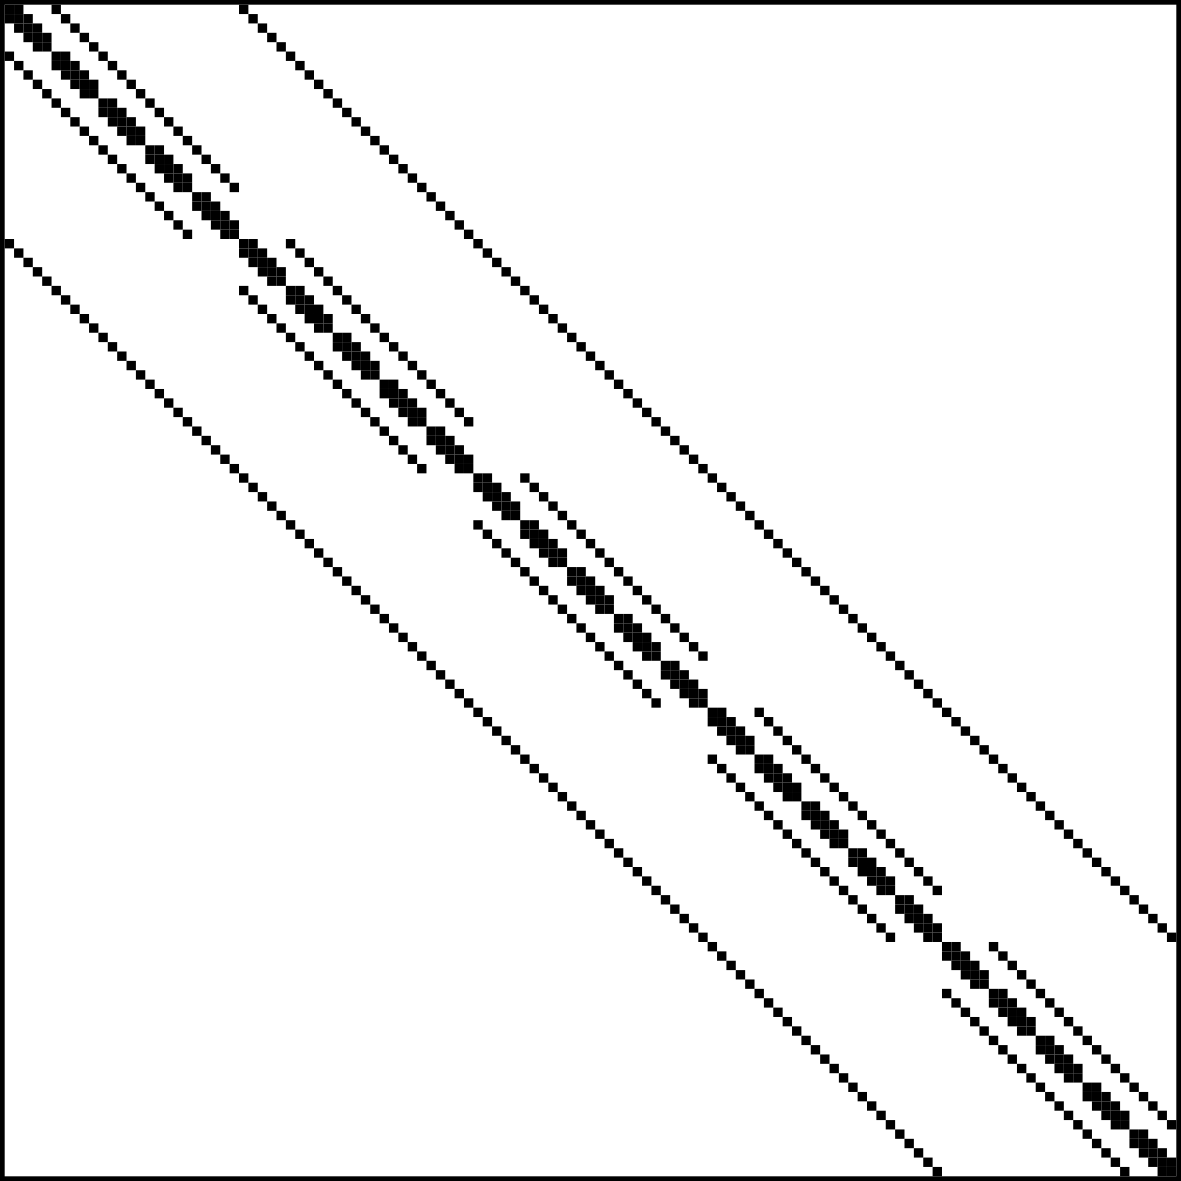
\includegraphics[width=0.9\textwidth]{fig/laplacian_example.png} % second figure itself
        \end{minipage}
        \caption[Structured grid and corresponding matrix for a simple Laplacian.]{\textbf{\bm{$5\times 5\times 5$} Structured grid and corresponding matrix for a simple Laplacian} $\nabla^2 u(\vec{r}) = 0$. The Laplace-operator is approximated by the conventional 3-axial symmetric discretization scheme, equivalent to a symmetric 7-point stencil operation.}
        \label{fig:laplacian-example}
    \end{figure}

    The solution procedure yields a sparse linear system whose solution is approximated by iterative methods involving
    repeated sparse matrix-vector-multiplications $Ax = b$ where the matrix $A$ encodes the adjacency structure of the
    grid. For a structured grid, the resulting matrix's distribution of non-zeros has a very distinct pattern. Generally
    speaking, such matrices consist of multiple diagonals of non-zero values at fixed intervals while all other elements
    are zero. The diagonals are almost fully dense with exceptions arising at positions corresponding to nodes at the
    grid's boundaries, where the regular adjacency pattern of the grid is disturbed by missing nodes. A grid and its
    corresponding sparse matrix's structure are depicted in Figure \ref{fig:laplacian-example} for a simple Laplacian
    problem.

    The matrix's non-zero values depend on the underlying physical problem's parameters, the type of PDE and the
    differential operators' discretization schemes. In general, the non-zeros' numeric values are independent of their
    location within the matrix but there exist classes of problems where where the presence of a matrix slice whose rows
    have diagonal structure implies that those rows share the same numeric values. Furthermore, solving problems on
    multiple coupled entities such as vectors or matrices yields sparse banded matrices whose 'elements' are themselves
    square matrices \cite{Godwin2013}.

    The sparse matrices relevant to this work are any sparse matrices that contain one or more sets of rows whose
    non-zero's column indices are identical save for a fixed offset. Sparse banded matrices arising from the procedure
    mentioned above have one such set to which the overwhelming majority of rows belong corresponding to all inner grid
    nodes (such as in the example in Figure \ref{fig:laplacian-example}). However, all of the ideas presented
    hereinafter may be applied to any sparse matrix whose structure exhibits any degree of repetitiveness.

    \Todo{Structured grid matrices expandieren}

    \chapter{3-Fold Compressed Sparse Row Matrix Storage Format}

  Evidently, representing a sparse banded matrix using the regular CSR format is suboptimal, as it provides no means of
  capturing the apparent repetitiveness of the structure. While at first glance the diagonal format might seem an
  appealing choice for the types of matrices introduced in the previous section, real-life problems produce matrices
  which are possibly only locally structured, i.e. they contain multiple fully structured sections corresponding to the
  multiple structured grid regions of the overall heterogeneous domain (Figure \ref{fig:refined_structured_grid}), which
  need not be aligned in a way to produce a diagonal structure at all. For such matrices the diagonal storage format is
  highly suboptimal \cite{Bell2011}. Thus a more flexible approach is taken adapting the general purpose CSR format to
  better suit the characteristics of sparse banded matrices.

  This section introduces the data layout and the matrix-vector multiplication scheme of the \keyword{3-fold compressed
  sparse row} matrix storage format (C3SR). Its raison d'être is to optimize arithmetic performance of matrix-vector
  multiplications involving sparse banded matrices by improving data locality through a structurally-aware space-saving
  storage scheme and by implementing an efficient arithmetic scheme capable of profiting from vectorization and
  multi-threading.

  \section{Data Layout and Storage Scheme}

    \Todo{Erläutern, dass 'structure of a matrix' die Positionen der Nonzeros und 'values' die numerischen Werte meint}

    It is crucial to observe that, in the most general case, a regularity inherent to a sparse banded matrix's
    non-zeros' column indices is not shared by the non-zeros' numerical values. While the non-zeros of two or more rows
    may share the same column indices, save for a possible offset, their corresponding values need not to be similar to
    each other at all. To prevent that a lack of common regularity impedes optimizing the storage of one or the other it
    is thus necessary to decouple the representation of a row's non-zeros' column index positions from the
    representation of their numerical values. The C3SR format accounts for this circumstance and maintains separate data
    structures for the non-zeros' column indices and their values. Hence the nomenclature of the C3SR format, as it is
    based on the idea of the CSR format and adds another two potential layers of compression: one for the column indices
    and one for the values.

    Based on the observation that sparse banded matrices contain many rows whose non-zeros are located at the same
    positions except for a possible offset the C3SR format decomposes the column index positions into the column index
    of the row's first non-zero element, referred to as the \keyword{row's peg} hereinafter, and the relative column
    indices of all of the row's non-zeros with respect to the first non-zero's column index, i.e. the relative offsets
    with respect to the peg index. The latter column index offsets relative to the peg index shall be called the
    \keyword{row's column index pattern}, or simply the \keyword{row's pattern}. Naturally, only unique patterns are stored,
    drastically shrinking the storage requirements of such matrices whose majority of rows exhibit the same pattern.

    Thus, in order to represent the column indices of a matrix row's non-zeros the C3SR format utilizes three arrays:

    \begin{description}[align = left, labelwidth = 4cm]
      \item [JP - \emph{Peg column indices}] \hfill \\
        Column index of each row's first non-zero. One element per row in matrix.
      \item [J - \emph{Column index patterns}] \hfill \\
        Column index position offsets of the rows' non-zeros relative to the peg
        column index for each row. Only unique patterns are stored.
      \item [JS - \emph{Patterns' index-pointers}] \hfill \\
        Index-pointer to each row's first element within J. One element per row in matrix.
    \end{description}

    An example matrix and its corresponding structural information are given in Figure \ref{fig:c3sr_example_structure}.

    \begin{figure}[ht]
      \centering
      \captionsetup{width=.9\textwidth}
      \begin{minipage}{0.4\textwidth}
        \centering
        $$
        \begin{pmatrix}
          0 & \bullet & 0 & \bullet & \bullet & 0 \\
          0 & \bullet & 0 & 0 & \bullet & 0 \\
          0 & 0 & \bullet & 0 & \bullet & \bullet \\
        \end{pmatrix}
        $$
      \end{minipage}
      \begin{minipage}{0.4\textwidth}
        \centering
        $$
        \begin{matrix}
          JP & : & 1 & 1 & 2 &   &   \\
           J & : & 0 & 2 & 3 & 0 & 3 \\
          JS & : & 0 & 3 & 0 &   &   \\
        \end{matrix}
        $$
      \end{minipage}
      \toccaption{Matrix with corresponding C3SR representation (structural information only).}{The non-zeros are
        denoted as black dots. The $0^{\text{th}}$ and $2^{\text{th}}$ row exhibit the same column index pattern
        $\big(0,2,3\big)$ at different peg index positions of $1$ and $2$, respectively. Thus the $0^{\text{th}}$ and
        the $2^{\text{th}}$ element of JS point J[0], which is the first element of this unique pattern. The
        $1^{\text{th}}$ row has a unique pattern which is stored after the previous pattern within J at offset $3$ which
        JS[1] accordingly points.}
      \label{fig:c3sr_example_structure}
    \end{figure}

    The matrix's non-zeros' numerical values are represented using two dense arrays: V, which contains the actual values
    and VS, the index-pointer into V which relates to V in the same way JS relates to J. As with J, row values are
    stored uniquely: Multiple rows with identical non-zeros (with possibly differing columns) lead to a single set of
    entries in V.

    \begin{description}[align = left, labelwidth = 4cm]
      \item [V - \emph{Values}] \hfill \\
        Non-zeros' numerical values. Duplicates across rows with the same pattern are stored only once.
      \item [VS - \emph{Values' index-pointers}] \hfill \\
        Index-pointer to each row's first element within V. One element per row in matrix.
    \end{description}

    An additional sixth array RS stores the number of non-zeros in each row of the matrix. This information is required
    as the index-pointer arrays JS and VS point a row's first element within J and V but, in contrast to the general CSR
    format, does not contain the information about how long the segment pertaining to the row within those arrays is. By
    virtue of the patterns' and values' storage schemes multiple rows' non-zeros' patterns and values may correspond to
    the very same portion of J and V such that the end of that portion cannot be retrieved from the corresponding
    index-pointer arrays JS and VS as could be done for the CSR format by taking the difference of two consecutive
    index-pointers from RP.

    \begin{description}[align = left, labelwidth = 4cm]
      \item [RS - \emph{Row sizes}] \hfill \\
        Number of non-zeros for each row. One element per row in matrix.
    \end{description}

    Another exemplary matrix and its full C3SR format representation are given in Figure \ref{fig:c3sr_example_full}.

    \begin{figure}[ht]
      \centering
      \begin{minipage}{0.4\textwidth}
        \centering
        $$
        \begin{pmatrix}
          1 & 2 & 0 & 3 & 0 & 0 \\
          0 & 1 & 2 & 0 & 3 & 0 \\
          0 & 0 & 4 & 5 & 0 & 0 \\
          0 & 0 & 6 & 7 & 0 & 0 \\
        \end{pmatrix}
        $$
      \end{minipage}
      \begin{minipage}{0.4\textwidth}
        \centering
        $$
        \begin{matrix}
          JP & : & 0 & 1 & 2 & 2 &   &   &   \\
           J & : & 0 & 1 & 3 & 0 & 1 &   &   \\
          JS & : & 0 & 0 & 3 & 3 &   &   &   \\
           V & : & 1 & 2 & 3 & 4 & 5 & 6 & 7 \\
          VS & : & 0 & 0 & 3 & 5 &   &   &   \\
          \RS & : & 3 & 3 & 2 & 2 &   &   &   \\
        \end{matrix}
        $$
      \end{minipage}
      \caption[Matrix with corresponding full C3SR representation.]{\textbf{Matrix with corresponding full C3SR representation.} The $0^{\text{th}}$ and $2^{\text{th}}$ rows exhibit the same pattern and the same values, thus the values are stored only once. The last two rows also share a common pattern but with different values.}
      \label{fig:c3sr_example_full}
    \end{figure}

    By design of the storage scheme, sparse banded matrices such as the example shown in Figure
    \ref{fig:laplacian-example} require very few elements within J as a structured grid's inner nodes, whose
    corresponding rows in the sparse banded matrix exhibit the same pattern which is only stored once, comprise the vast
    majority of all nodes. Depending on the underlying physical problem this property also applies to V if all rows of
    an equal pattern share the same set of values. 

    As will be detailed in the following section \ref{subsec:matrix-vector-multiplication-schemes} a matrix-vector
    multiplication involves copiously accessing J and V. The C3SR format greatly improves the spatial locality of the
    data fields most relevant to arithmetic. A best-case example is given in Figure \ref{fig:c3sr-example-best-case}.

    \begin{figure}[ht]
      \centering
      \begin{minipage}{0.5\textwidth}
        \centering
        $$
        \begin{pmatrix}
          1 & 0 & 2 & 0 & 3 & 4 & 0 & 0 & 0 & 0 \\
          0 & 1 & 0 & 2 & 0 & 3 & 4 & 0 & 0 & 0 \\
            &   & \ddots &   & \ddots &   & \ddots & \ddots \\
          0 & 0 & 0 & 1 & 0 & 2 & 0 & 3 & 4 & 0 \\
          0 & 0 & 0 & 0 & 1 & 0 & 2 & 0 & 3 & 4 \\
        \end{pmatrix}
        $$
      \end{minipage}
      \begin{minipage}{0.4\textwidth}
        \centering
        $$
        \begin{matrix}
          JP & : & 0 & 1 & 2 & 3 & \cdots & N-1 \\
           J & : & 0 & 2 & 4 & 5 &        &     \\
          JS & : & 0 & 0 & 0 & 0 & \cdots &  0  \\
           V & : & 1 & 2 & 3 & 4 &        &     \\
          VS & : & 0 & 0 & 0 & 0 & \cdots &  0  \\
          \RS & : & 4 & 4 & 4 & 4 & \cdots &  4  \\
        \end{matrix}
        $$
      \end{minipage}
      \caption[Best-case sparse matrix with corresponding C3SR representation.]{\textbf{Best-case sparse matrix with corresponding C3SR representation.} The matrix exhibits a single pattern and all of its rows have the same values leading to minimally sized J and V optimal for the repeated accesses required for matrix-vector multiplication.}
      \label{fig:c3sr-example-best-case}
    \end{figure}

    Note that the structure of a sparse banded matrix derived from a fully structured grid is exclusively diagonal or
    locally uniform, i.e. the non-zeros either align into multiple diagonals as in Figure \ref{fig:laplacian-example} or
    contain blocks of square matrices when solving for multiple coupled entities. Thus the concept of decomposing a
    row's non-zeros' column indices into its peg index and patterns is slightly redundant but is retained for the sake
    of flexibility when dealing with matrices associated with grids which contain structured segments. \Todo{Absatz
    rausschmeißen?}

    \Todo{Prämisse der korrekten Indizierung der Gitterknoten explizit betonen.}

  \section{Matrix-Vector Multiplication Schemes} \label{subsec:matrix-vector-multiplication-schemes}

    Aside from the basic CSR-like matrix-vector multiplication scheme, the C3SR format's storage scheme allows for a
    vectorized arithmetic scheme for sparse banded matrices. This section details the different matrix-vector
    multiplication schemes whose performance is then gauged in the subsequent section.

    \Todo{Nomenklatur 'scalar' für CSR-Schema einführen und verwenden}

    \subsection{Basic CSR-like Multiplication Scheme} \label{subsubsec:basic-csr-like-multiplication-scheme}

      Algorithmically, the basic row-by-column matrix-vector multiplication scheme of the C3SR format is similar to that
      of the CSR format. Differences arise only in the C3SR's additional offset $JP[k]$ which is applied to each
      relative column index prior to accessing the argument vector $x$ as shown in Figure
      \ref{fig:csr-vs-c3sr-mvm-scalar}.

      \begin{figure}[ht]
        \centering
        \captionsetup{width=0.9\columnwidth}
        $$
\begin{matrix}
  \text{CSR}  & : & \sum \limits_{\alpha = 0}^{\RP[k+1] - \RP[k] - 1} & \bigg( & V[\RP[k] + \alpha]   & \cdot & x\big[\CI[\RP[k] + \alpha]\big] & \bigg)\\
  \vspace{0.3cm} \\
  \text{C3SR} & : & \sum \limits_{\alpha = 0}^{\RS[k] - 1} & \bigg( & V\big[VS[k] + \alpha\big] & \cdot & x\bigg[J\big[JS[k] + \alpha\big] + JP[k]\bigg] & \bigg) \\
\end{matrix}
$$

        \toccaption{Matrix-vector multiplication schemes of the C3SR and CSR format in comparison.}
        {The $k^{\text{th}}$ component of the product $Ax$ is shown. The C3SR format accesses V and J from their
        dedicated index-pointer arrays while the CSR format utilizes one common row-pointer array \RP. Additionally, the
        C3SR format requires the relative column indices to be offset by the peg column index for each row.}
        \label{fig:csr-vs-c3sr-mvm-scalar}
      \end{figure}

      As the C3SR format utilizes additional arrays to store index-pointers the number of memory accesses increases
      likewise. Assuming a general case of a large sparse matrix devoid of any regularity in its structure whose size
      exceeds the machine's cache capacity the CSR format's arithmetic performance will be better proportional to the
      difference in the storage size as the above schemes yield memory bound computations involving few trivial
      arithmetic operations.

      On the flipside, as demonstrated in the previous section sparse banded matrices facilitate very compact storage
      allowing a small segment of memory, corresponding to possibly only a few cache lines, to contain the matrix's
      complete structural information and, depending on the underlying physical problem, even the numeric values. This
      can drastically improve the arithmetic performance of the C3SR format despite the more complex memory access
      scheme as will be shown in the benchmark section.

    \subsection{Vectorized SIMD Multiplication Scheme} \label{subsubsec:vectorized-simd-multiplication-scheme}

      Aside of the performance benefits due to smaller object sizes and better data locality sparse banded matrices
      derived from structured grids stored in C3SR-format exhibit data layouts particularly well suited for a vectorized
      implementation of matrix-vector multiplication.

      Seeing as the standard CSR-format's implementation of sparse matrix-vector multiplication is a memory-bound
      operation for large matrices which necessitates loading data from main memory, the drastic decrease in object size
      when applying the C3SR-format's compression scheme can reduce the object size enough for it to fit into cache
      memory whose higher bandwidth may allow to increase arithmetic performance through vectorization. Such
      benefits are verified in the benchmark section\Todo{Add reference to mvm}.

      Depending on the source matrix's structure and values its data is laid out in memory such that matrix-vector
      multiplication can be performed simultaneously for multiple rows using vectorization. Several configurations of
      the values and the structure of a matrix slice, for which the matrix-vector multiplication can be vectorized,
      exist and arise in real-world applications. The configurations require similar data access patterns and
      implementations which shall be presented here alongside their corresponding matrix slice. The different
      implementations will be referred to as \keyword{SIMD schemes}.

      \subsubsection{Matrix Slice Compositions and corresponding SIMD Schemes}

        For the implementation of vectorized matrix-vector multiplication for a matrix slice its non-zeros' values are
        assigned one of two categories: If all rows share the same values in the same order of the appearance of
        non-zeros in the row, the values' composition is referred to as \keyword{collated}, named after the fact that by
        virtue of the C3SR-format's storage scheme said set of values is stored only once in memory, hence collating the
        values for all rows in the matrix slice into a single segmment. Note that the non-zeros' column indices are of
        no concern here and may differ between rows as long as the values are identical. Conversely, if the matrix
        slice's values are not collated it's composition is referred to as \keyword{arbitrary}.

        Similarly to a matrix slice's values its structure falls into one of three categories: If the non-zeros are
        aligned in dense diagonals its structure is referred to as \keyword{diagonal}. A \keyword{uniform} structure is
        present if all non-zeros are aligned into vertical columns, i.e. every row's non-zeros share the same column
        indices. Finally, if the matrix slice's structural composition is neither diagonal nor uniform, it is assigned
        the default of \keyword{arbitrary}.

        Thus a total of $2 \times 3 = 6$ different data access patterns and implementations are considered, arising from
        all possible combinations of the values' and the structural compositions. For the sake of brevity a tuple of a
        matrix slice's values' composition and its structural composition shall be referred to as the \keyword{slice's
        composition}. Each variant of slice composition is detailed in the following paragraphs along with its data
        access patterns required to vectorize matrix-vector multiplication.

        Note that the concepts introduced herein are generic and apply to matrix slices with arbitrary numbers of rows.
        A specific choice of the number of rows in a slice must depend on the underlying hardware's vector register size
        and is further detailed in the corresponding implementation section (see \Todo{Ref impl:mvm-vectorized}). This
        section serves to introduce the basic idea.

        \Todo{Architekturen mit schneller Stride-Gather Instruktion suchen}

        \Todo{Slice Composition hängt von genauer Datenpositionierung ab und kann nicht ausschließlich aus dem Slice
        bestimmt werden. Frühere Reihen könnten selbe Values gehabt haben, was aber Sonderfall ist. Slicecompo wird aus
        tatsächlichem Datenlayout bestimmt und nicht aus der Teilmatrix, daher nono}

        \paragraph{SIMD Scheme I: Arbitrary Values \& Diagonal Structure}

          Suppose that a horizontal slice of rows $r, \ldots, r+k$ has a diagonal structure with the diagonals starting
          at indices $s, t, \ldots $, such as is depicted in the upper segment of Figure
          \ref{fig:simd-scheme-i-data-layout}. The matrix-vector multiplication for each of the slice's rows is composed
          of the same number of summands, one per diagonal. Each of the summands is a product of the diagonal's non-zero
          entry and the argument's corresponding element, starting out with $a_{r,s} \cdot x_s$ for the first diagonal's
          initial element and $a_{r,t} \cdot x_t$ for the second diagonal. For each subsequent row the matrix element's
          indices are incremented as well as the argument vector's index, commencing with $a_{r+1, s+1} \cdot x_{s+1}$
          for the first diagonal's second element and accordingly for each other diagonal.

          \begin{figure}[H]
            \centering
            \captionsetup{width=0.9\columnwidth}
            $$
\begin{bNiceMatrix}[first-row, last-col=13, code-for-first-row=\color{blue}, code-for-last-col=\color{blue}]
         & s-1    & s       & s+1         & s+ 2        & s+ 3   &        & t       & t+1         & t+2         & t+3    &        & \\
\cdots   & 0      & a_{r,s} & 0           & \cdots      & \cdots & \cdots & a_{r,t} & 0           & \cdots      & \cdots & \cdots & r     \\
\cdots   & \cdots & 0       & a_{r+1,s+1} & 0           & \cdots & \cdots & \cdots  & a_{r+1,t+1} & 0           & \cdots & \cdots & r+1   \\
\cdots   & \cdots & \cdots  & 0           & a_{r+2,s+2} & 0      & \cdots & \cdots  & \cdots      & a_{r+2,t+2} & 0      & \cdots & r+ 2  \\
\end{bNiceMatrix}
$$

\begin{tikzpicture}[
  show background rectangle,
  node distance=1cm and 0.1cm,
  vsstyle/.style={inner sep=0, outer sep=0, draw=gray, fill=dodgerblue4, text=white, minimum height=1cm, minimum width=2cm},
  vstyle/.style={draw=gray, inner sep=0, outer sep=0, minimum height=1cm, minimum width=2cm},
  namestyle/.style={draw=none, minimum height=1cm, minimum width=1cm},
  m/.style={minimum height=0.5cm, minimum width=1cm, text height=1.5ex, text depth=0.25ex, yshift=0.5mm}, % Matrix entries
  ml/.style={text=red, minimum width=1cm, anchor=base},
  dotstyle/.style={draw=none, minimum height=0, minimum width=0},
  pathstyle/.style={->}
]

% TODO: Use \coodinate instead of empty \node.
  %%% Matrix

  % Reference colummn to fix y-offset between rows. Shit's fucked.
  \node[]                            (R0) {};
  \node[] at ($(R0.south)+(0,-6mm)$) (R1) {};
  \node[] at ($(R1.south)+(0,-4mm)$) (R2) {};
  \node[] at ($(R2.south)+(0,-4mm)$) (R3) {};

  % Col 0
  \node[ml] (R0C0) at (R0)         {$$};
  \node[m]  (R1C0) at (R1 -| R0C0) {$\cdots$};
  \node[m]  (R2C0) at (R2 -| R0C0) {$\cdots$};
  \node[m]  (R3C0) at (R3 -| R0C0) {$\cdots$};

  % Col 1
  \node[ml, right=of R0] (R0C1)                 {$s-1$};
  \node[m]               (R1C1) at (R1 -| R0C1) {$0$};
  \node[m]               (R2C1) at (R2 -| R0C1) {$\cdots$};
  \node[m]               (R3C1) at (R3 -| R0C1) {$\cdots$};

  % Col 2
  \node[ml, right=of R0C1] (R0C2)                 {$s$};
  \node[m]                 (R1C2) at (R1 -| R0C2) {$a_{r,s}$};
  \node[m]                 (R2C2) at (R2 -| R0C2) {$0$};
  \node[m]                 (R3C2) at (R3 -| R0C2) {$\cdots$};

  % Col 3
  \node[ml, right=of R0C2] (R0C3)                 {$s+1$};
  \node[m]                 (R1C3) at (R1 -| R0C3) {$0$};
  \node[m]                 (R2C3) at (R2 -| R0C3) {$a_{r+1, s+1}$};
  \node[m]                 (R3C3) at (R3 -| R0C3) {$0$};

  % Col 4
  \node[ml, right=of R0C3] (R0C4)                 {$s+2$};
  \node[m]                 (R1C4) at (R1 -| R0C4) {$\cdots$};
  \node[m]                 (R2C4) at (R2 -| R0C4) {$0$};
  \node[m]                 (R3C4) at (R3 -| R0C4) {$a_{r+2, s+2}$};

  % Col 5
  \node[ml, right=of R0C4] (R0C5)                 {$s+3$};
  \node[m]                 (R1C5) at (R1 -| R0C5) {$\cdots$};
  \node[m]                 (R2C5) at (R2 -| R0C5) {$\cdots$};
  \node[m]                 (R3C5) at (R3 -| R0C5) {$0$};

  % Col 6
  \node[ml, right=of R0C5] (R0C6)                 {$\cdots$};
  \node[m]                 (R1C6) at (R1 -| R0C6) {$\cdots$};
  \node[m]                 (R2C6) at (R2 -| R0C6) {$\cdots$};
  \node[m]                 (R3C6) at (R3 -| R0C6) {$\cdots$};

  % Col 7
  \node[ml, right=of R0C6] (R0C7)                 {$t$};
  \node[m]                 (R1C7) at (R1 -| R0C7) {$a_{r,t}$};
  \node[m]                 (R2C7) at (R2 -| R0C7) {$\cdots$};
  \node[m]                 (R3C7) at (R3 -| R0C7) {$\cdots$};

  % Col 8
  \node[ml, right=of R0C7] (R0C8)                 {$t+1$};
  \node[m]                 (R1C8) at (R1 -| R0C8) {$0$};
  \node[m]                 (R2C8) at (R2 -| R0C8) {$a_{r+1, t+1}$};
  \node[m]                 (R3C8) at (R3 -| R0C8) {$\cdots$};

  % Col 9
  \node[ml, right=of R0C8] (R0C9)                 {$t+2$};
  \node[m]                 (R1C9) at (R1 -| R0C9) {$\cdots$};
  \node[m]                 (R2C9) at (R2 -| R0C9) {$0$};
  \node[m]                 (R3C9) at (R3 -| R0C9) {$a_{r+2,t+2}$};

  % Col 10
  \node[ml, right=of R0C9] (R0C10)                  {$t+3$};
  \node[m]                 (R1C10) at (R1 -| R0C10) {$\cdots$};
  \node[m]                 (R2C10) at (R2 -| R0C10) {$\cdots$};
  \node[m]                 (R3C10) at (R3 -| R0C10) {$0$};

  % Col 11
  \node[ml, right=of R0C10] (R0C11)                  {$\cdots$};
  \node[m]                  (R1C11) at (R1 -| R0C11) {$\cdots$};
  \node[m]                  (R2C11) at (R2 -| R0C11) {$\cdots$};
  \node[m]                  (R3C11) at (R3 -| R0C11) {$\cdots$};

  % Col 12
  \node[ml, right=of R0C11] (R0C12)                  {};
  \node[ml]                 (R1C12) at (R1 -| R0C12) {$r$};
  \node[ml]                 (R2C12) at (R2 -| R0C12) {$r+1$};
  \node[ml]                 (R3C12) at (R3 -| R0C12) {$r+2$};

  % Separator lines
  \node (SEP-HORIZ-L) at ($(R0C0.south west)!0.5!(R1C0.north west)$) {};
  \node (SEP-HORIZ-R) at (SEP-HORIZ-L -| R0C12.east) {};
  \draw[draw=gray, line width=0.3mm] (SEP-HORIZ-L) -- (SEP-HORIZ-R);
  \node (SEP-VERT-T) at ($(R0C11.north east)!0.5!(R0C12.north west)$) {};
  \node (SEP-VERT-B) at (SEP-VERT-T |- R3C11.south east) {};
  \draw[draw=gray, line width=0.3mm] (SEP-VERT-T) -- (SEP-VERT-B);

  % matrix bounding box edges
  \node (MAT-TL) at (R0C0.north west) {};
  \node (MAT-BL) at (R3C0.south west) {};
  \def\gutterThickness{5mm}
  \def\gutterYPadding{2mm}
  \def\gutterGap{2mm}
  \def\gutterColor{gray}
  \def\matrixDistToGutter{10mm} % Horizontal distance between matrix & gutter
  \node (GUTTER-MAT-TR) at ($(MAT-TL)+(-\matrixDistToGutter,\gutterYPadding)$) {};
  \node (GUTTER-MAT-BR-CHECKPT) at (GUTTER-MAT-TR |- MAT-BL) {};
  \node (GUTTER-MAT-BR) at ($(GUTTER-MAT-BR-CHECKPT)+(0,-\gutterYPadding)$) {};
  \node (GUTTER-MAT-BL) at ($(GUTTER-MAT-BR)+(-\gutterThickness,0)$) {};
  \fill[fill=\gutterColor] (GUTTER-MAT-TR) rectangle (GUTTER-MAT-BL);
  \node[text=white] at ($(GUTTER-MAT-TR)!0.5!(GUTTER-MAT-BL)$) {I};

  %%% Data Layout

  \def\dataDistToGutter{2mm}
  \node (GUTTER-DATA-TR) at ($(GUTTER-MAT-BR)+(0,-\gutterGap)$) {};
  \node[] (DATA-TL) at ($(GUTTER-DATA-TR)+(\dataDistToGutter,-\gutterYPadding)$) {};

  \node[namestyle, anchor=north west] at (DATA-TL) (VNAME)
    {V};
  \node[namestyle, below=of VNAME] (VSNAME)
    {VS};
  \node[namestyle, below=of VSNAME] (JNAME)
    {J};
  \node[namestyle, below=of JNAME] (JSNAME)
    {JS};
  \node[namestyle, below=of JSNAME] (JPNAME)
    {JP};
  \node[vstyle, right=of VNAME] (V1)
    {$a_{r,s}$};

  \node[vstyle, right=of V1] (V2)
    {$a_{r,t}$};
  \node[dotstyle, right=2mm of V2] (V3)
    {$\cdots$};
  \node[vstyle, right=2mm of V3] (V4)
    {$a_{r+1,s+1}$};
  \node[vstyle, right=of V4] (V5)
    {$a_{r+1,t+1}$};
  \node[dotstyle, right=2mmof V5] (V6)
    {$\cdots$};
  \node[vstyle, right=2mm of V6] (V7)
    {$a_{r+2,s+2}$};
  \node[vstyle, right=of V7] (V8)
    {$a_{r+2,t+2}$};
  \node[dotstyle, right=2mm of V8] (V9)
    {$\cdots$};

  \node[vsstyle, below=of V1] (VS1)
    {};
  \node[vsstyle, right=of VS1] (VS2)
    {};
  \node[vsstyle, right=of VS2] (VS3)
    {};

  \node[vstyle, below=of VS1] (J1)
    {$0$};
  \node[vstyle, right=of J1] (J2)
    {$(t-s)$};
  \node[dotstyle, right=2mm of J2] (J3)
    {$\cdots$};

  \node[vsstyle, below=of J1] (JS1)
    {};
  \node[vsstyle, right=of JS1] (JS2)
    {};
  \node[vsstyle, right=of JS2] (JS3)
    {};

  \node[vstyle, below=of JS1] (JP1)
    {$s$};
  \node[vstyle, right=of JP1] (JP2)
    {$s+1$};
  \node[vstyle, right=of JP2] (JP3)
    {$s+2$};

  \draw[pathstyle] (VS1.north) |- ($(VS1.north)!0.5!(V1.south)$) -| (V1.south);
  \draw[pathstyle] (VS2.north) |- ($(VS2.north)!0.66!(V4.south)$) -| (V4.south);
  \draw[pathstyle] (VS3.north) |- ($(VS3.north)!0.33!(V7.south)$) -| (V7.south);

  \draw[pathstyle] (JS1.north) |- ($(JS1.north)!0.25!(J1.south)$) -| ($(J1.south)-(3mm,0)$);
  \draw[pathstyle] (JS2.north) |- ($(JS2.north)!0.50!(J1.south)$) -| ($(J1.south)-(0mm,0)$);
  \draw[pathstyle] (JS3.north) |- ($(JS3.north)!0.75!(J1.south)$) -| ($(J1.south)+(3mm,0)$);

  %% Data gutter

  \node (DATA-BL) at (JPNAME.south west -| DATA-TL) {};
  \node (GUTTER-DATA-BR-CHECKPT) at (GUTTER-DATA-TR |- DATA-BL) {};
  \node (GUTTER-DATA-BR) at ($(GUTTER-DATA-BR-CHECKPT)+(0, -\gutterYPadding)$) {};
  \node (GUTTER-DATA-BL) at ($(GUTTER-DATA-BR)+(-\gutterThickness, 0)$) {};
  \fill[fill=\gutterColor] (GUTTER-DATA-TR) rectangle (GUTTER-DATA-BL);
  \node[text=white] (GUTTER-II) at ($(GUTTER-DATA-BL)!0.5!(GUTTER-DATA-TR)$) {II};

   % \fill[fill=\gutterColor] 
%   \def\gutterThickness{5mm}
%   \def\gutterYPadding{2mm}
%   \def\gutterGap{2mm}
%   \node (GUTTER-MAT-TR) at ($(R0C0.north west)+(0,\gutterYPadding)$) {};
%   \node (GUTTER-MAT-BL) at ($(R3C0.south west)-(\gutterThickness,\gutterYPadding)$) {};
%   \node (GUTTER-MAT-BR) at ($(GUTTER-MAT-BL)+(\gutterThickness,0)$) {};
%   \fill[fill=gray] (GUTTER-MAT-TR) rectangle (GUTTER-MAT-BL);
%   \node[text=white] at ($(GUTTER-MAT-TR)!0.5!(GUTTER-MAT-BL)$) {I};
% 
%   %%% Data Layout
% 
%   \node (GUTTER-DATA-TR) at ($(GUTTER-MAT-BR)+(0,-\gutterGap)$) {};
%   \node[] (DATA-TL) at ($(GUTTER-DATA-TR)+(0,-\gutterYPadding)$) {};


\end{tikzpicture}

$$
\begin{matrix}
  \begin{bmatrix}
    a_{r,s}     \\
    a_{r+1,s+1} \\
       \vdots   \\
    a_{r+k,s+k} \\
  \end{bmatrix} & \cdot & \begin{bmatrix}
                            x_s      \\
                            x_{s+1}  \\
                              \vdots \\
                            x_{s+k}  \\
                          \end{bmatrix} & + & \begin{bmatrix}
                                              a_{r,t}     \\
                                              a_{r+1,t+1} \\
                                                \vdots    \\
                                              a_{r+k,t+k} \\
                                              \end{bmatrix} & \cdot & \begin{bmatrix}
                                                                        x_t \\
                                                                        x_{t+1} \\
                                                                        \vdots \\
                                                                        x_{t+k}
                                                                      \end{bmatrix} & + & \cdots & = \begin{bmatrix}
                                                                                                         y_{r} \\
                                                                                                         y_{r+1} \\
                                                                                                         \vdots \\
                                                                                                         y_{r+k}
                                                                                                        \end{bmatrix}\\

\end{matrix}
$$

            \toccaption{Matrix slice with arbitrary values and diagonal structure, corresponding data layout and
              arithmetic scheme.}{Section I shows a matrix slice with arbitrary values and diagonal structure. Row and
              column indices are indicated at the matrix's perimeter. Section II displays the slice's corresponding data
              layout. Index-pointer values are indicated by arrows to the elements they point. Only arrays relevant to
              the arithmetic scheme are sketched. Section III shows the arithmetic scheme for a slice of $k$ rows which
              is translated into operations on vector registers.}
            \label{fig:simd-scheme-i-data-layout}
          \end{figure}

          As each diagonal's summand accesses the argument vector's elements in consecutive fashion, for example, $x_s,
          x_{s+1}, \ldots, x_{s + k}$ for the first diagonal, the access to the argument vector's elements can be
          vectorized. The other summand's constituents, the diagonal's elements, are stored within V at a fixed stride
          which is equal to the number of diagonals. This is due to the fact that the matrix slice's non-zero elements
          are stored row-by-row while each row has the same number of elements. Thus, for the general case when the
          rows' values don't match, $a_{r, s}$ is located as many elements before $a_{r+1, s+1}$ within V as there are
          diagonals.

          In SIMD terms a stride-gather and a load are required for the diagonal's elements and the argument vector,
          respectively. The two vector registers are then multiplied and the result is then added onto the next product
          pertaining to the subsequent diagonal. After the final vectorized addition the result is written into the
          output buffer using a vectorized store. Figure \ref{fig:simd-scheme-i-data-layout} shows the matrix's data
          layout in memory and the arithmetic scheme.

        \paragraph{SIMD Scheme II: Collated Values \& Diagonal Structure}

          The second SIMD scheme applies to matrix slice with collated values and diagonal structure. As all values
          within a diagonal are identical, e.g. $a_{r,s} = a_{r+1, s+1} = \ldots$ for the first diagonal, the arithmetic
          is simplified with respect to the previous scheme. Instead of being subjected to a vectorized multiplication,
          the argument vector's values are simply scaled by the diagonal's value. Figure \ref{fig:simd-scheme-ii-data-layout})
          shows the data layout and arithmetic scheme resulting from this configuration.

          \begin{figure}[H]
            \centering
            \captionsetup{width=0.9\columnwidth}
            $$
\begin{bNiceMatrix}[first-row, last-col=13, code-for-first-row=\color{blue}, code-for-last-col=\color{blue}]
          & s-1    & s      & s+1    & s+2    & s+3    &        & t      & t+1    & t+2    & t+3    &        & \\
\cdots    & 0      & \alpha & 0      & \cdots & \cdots & \cdots & \beta  & 0      & \cdots & \cdots & \cdots & r     \\
\cdots    & \cdots & 0      & \alpha & 0      & \cdots & \cdots & \cdots & \beta  & 0      & \cdots & \cdots & r+1   \\
\cdots    & \cdots & \cdots & 0      & \alpha & 0      & \cdots & \cdots & \cdots & \beta  & 0      & \cdots & r+ 2  \\
\end{bNiceMatrix}
$$

\begin{tikzpicture}[
  node distance=1cm and 0.1cm,
  vsstyle/.style={inner sep=0, outer sep=0, draw=gray, fill=dodgerblue4, text=white, minimum height=1cm, minimum width=2cm},
  vstyle/.style={draw=gray, inner sep=0, outer sep=0, minimum height=1cm, minimum height=1cm, minimum width=2cm},
  namestyle/.style={draw=none, minimum height=0, minimum width=1cm},
  dotstyle/.style={draw=none, minimum height=0, minimum width=0},
  pathstyle/.style={->}
]

  \node[vstyle] (V1)
    {$\alpha$};
  \node[vstyle, right=of V1] (V2)
    {$\beta$};
  \node[dotstyle, right=2mm of V2] (V3)
    {$\cdots$};

  \node[vsstyle, below=of V1] (VS1)
    {};
  \node[vsstyle, right=of VS1] (VS2)
    {};
  \node[vsstyle, right=of VS2] (VS3)
    {};

  \node[vstyle, below=of VS1] (J1)
    {$0$};
  \node[vstyle, right=of J1] (J2)
    {$(t-s)$};
  \node[dotstyle, right=2mm of J2] (J3)
    {$\cdots$};

  \node[vsstyle, below=of J1] (JS1)
    {};
  \node[vsstyle, right=of JS1] (JS2)
    {};
  \node[vsstyle, right=of JS2] (JS3)
    {};

  \node[vstyle, below=of JS1] (JP1)
    {$s$};
  \node[vstyle, right=of JP1] (JP2)
    {$s+1$};
  \node[vstyle, right=of JP2] (JP3)
    {$s+2$};

  \node[namestyle, left=of V1] (VNAME)
    {V};
  \node[namestyle, left=of VS1] (VSNAME)
    {VS};
  \node[namestyle, left=of J1] (JNAME)
    {J};
  \node[namestyle, left=of JS1] (JSNAME)
    {JS};
  \node[namestyle, left=of JP1] (JPNAME)
    {JP};

  \draw[pathstyle] (VS1.north) |- ($(VS1.north)!0.25!(V1.south)$) -| ($(V1.south)-(3mm,0)$);
  \draw[pathstyle] (VS2.north) |- ($(VS2.north)!0.50!(V1.south)$) -| ($(V1.south)-(0mm,0)$);
  \draw[pathstyle] (VS3.north) |- ($(VS3.north)!0.75!(V1.south)$) -| ($(V1.south)+(3mm,0)$);

  \draw[pathstyle] (JS1.north) |- ($(JS1.north)!0.25!(J1.south)$) -| ($(J1.south)-(3mm,0)$);
  \draw[pathstyle] (JS2.north) |- ($(JS2.north)!0.50!(J1.south)$) -| ($(J1.south)-(0mm,0)$);
  \draw[pathstyle] (JS3.north) |- ($(JS3.north)!0.75!(J1.south)$) -| ($(J1.south)+(3mm,0)$);
\end{tikzpicture}


$$
\begin{matrix}
 \alpha & \cdot & \begin{bmatrix}
                            x_s      \\
                            x_{s+1}  \\
                              \vdots \\
                            x_{s+k}  \\
  \end{bmatrix} & + & \beta & \cdot & \begin{bmatrix}
                                        x_t \\
                                        x_{t+1} \\
                                        \vdots \\
                                        x_{t+k}
                                                                      \end{bmatrix} & + & \cdots & =  \begin{bmatrix}
                                                                                                         y_{r} \\
                                                                                                         y_{r+1} \\
                                                                                                         \vdots \\
                                                                                                         y_{r+k}
                                                                                                        \end{bmatrix}
\end{matrix}
$$

            \toccaption{Matrix slice with collated values and diagonal structure, corresponding data layout and
              arithmetic scheme.}{Section I shows a matrix slice with collated values and diagonal structure. Row and
              column indices are indicated at the matrix's perimeter. Section II displays the slice's corresponding data
              layout. Index-pointer values are indicated by arrows to the elements they point. Only arrays relevant to
              the arithmetic scheme are sketched. Section III shows the arithmetic scheme for a slice of $k$ rows which
              is translated into operations on vector registers.}
            \label{fig:simd-scheme-ii-data-layout}
          \end{figure}

        \paragraph{SIMD Scheme III: Arbitrary Values \& Uniform Structure}

          The third SIMD scheme may arise when solving PDEs on coupled entities producing matrix slices of uniform
          structure and arbitrary values. This leads to the circumstance that the argument vector's element required for
          the partial sum involving a matrix column is constant for the whole column as outlined in Figure
          \ref{fig:simd-scheme-iii-data-layout}. Thus the argument vector's elements serve as scaling constants for the
          vector register containing the matrix's elements which, as in the first configuration, are spread at a fixed
          stride throughout V.

          \begin{figure}[H]
            \centering
            \captionsetup{width=0.9\columnwidth}
            \begin{tikzpicture}[
  show background rectangle,
  node distance=5mm and 0.1cm,
  vsstyle/.style={inner sep=0, outer sep=0, draw=gray, fill=dodgerblue4, text=white, minimum height=1cm, minimum width=2cm},
  vstyle/.style={draw=gray, inner sep=0, outer sep=0, minimum height=1cm, minimum width=2cm},
  namestyle/.style={draw=none, minimum height=1cm, minimum width=1cm},
  m/.style={minimum height=0.5cm, minimum width=1cm, text height=1.5ex, text depth=0.25ex, yshift=0.5mm}, % Matrix entries
  ml/.style={text=red, minimum height=0.5cm, minimum width=1cm, anchor=base},
  dotstyle/.style={draw=none, minimum height=0, minimum width=0},
  pathstyle/.style={->}
]

  %%% Matrix

  \def\gutterThickness{5mm} % width of gutter
  \def\gutterYPadding{2mm} % Vertical extension of gutter beyond heigh of its section's content
  \def\gutterGap{2mm} % Vertical gap between gutter sections
  \def\gutterColor{gray} % Gutter fill color
  \def\matrixDistToGutter{30mm} % Horizontal distance between matrix & gutter
  \def\schemeDistToGutter{30mm} % Horizontal distance between scheme & gutter

  % Reference colummn to fix y-offset between rows. Shit's fucked.
  \node[] (R0)                            {};
  \node[] (R1) at ($(R0.south)+(0,-6mm)$) {};
  \node[] (R2) at ($(R1.south)+(0,-4mm)$) {};
  \node[] (R3) at ($(R2.south)+(0,-4mm)$) {};

  % Col 0
  \node[ml] (R0C0) at (R0)         {$\cdots$};
  \node[m]  (R1C0) at (R1 -| R0C0) {$\cdots$};
  \node[m]  (R2C0) at (R2 -| R0C0) {$\cdots$};
  \node[m]  (R3C0) at (R3 -| R0C0) {$\cdots$};

  % Col 1
  \node[ml, right=of R0C0] (R0C1)                 {$s-1$};
  \node[m]                 (R1C1) at (R1 -| R0C1) {$0$};
  \node[m]                 (R2C1) at (R2 -| R0C1) {$0$};
  \node[m]                 (R3C1) at (R3 -| R0C1) {$0$};

  % Col 2
  \node[ml, right=of R0C1] (R0C2)                 {$s$};
  \node[m]                 (R1C2) at (R1 -| R0C2) {$a_{r,s}$};
  \node[m]                 (R2C2) at (R2 -| R0C2) {$a_{r+1,s}$};
  \node[m]                 (R3C2) at (R3 -| R0C2) {$a_{r+2,s}$};

  % Col 3
  \node[ml, right=of R0C2] (R0C3)                 {$s+1$};
  \node[m]                 (R1C3) at (R1 -| R0C3) {$0$};
  \node[m]                 (R2C3) at (R2 -| R0C3) {$0$};
  \node[m]                 (R3C3) at (R3 -| R0C3) {$0$};

  % Col 4
  \node[ml, right=of R0C3] (R0C4)                 {$\cdots$};
  \node[m]                 (R1C4) at (R1 -| R0C4) {$\cdots$};
  \node[m]                 (R2C4) at (R2 -| R0C4) {$\cdots$};
  \node[m]                 (R3C4) at (R3 -| R0C4) {$\cdots$};

  % Col 5
  \node[ml, right=of R0C4] (R0C5)                 {$t$};
  \node[m]                 (R1C5) at (R1 -| R0C5) {$a_{r,t}$};
  \node[m]                 (R2C5) at (R2 -| R0C5) {$a_{r+1,t}$};
  \node[m]                 (R3C5) at (R3 -| R0C5) {$a_{r+2,t}$};

  % Col 6
  \node[ml, right=of R0C5] (R0C6)                 {$t+1$};
  \node[m]                 (R1C6) at (R1 -| R0C6) {$0$};
  \node[m]                 (R2C6) at (R2 -| R0C6) {$0$};
  \node[m]                 (R3C6) at (R3 -| R0C6) {$0$};

  % Col 7
  \node[ml, right=of R0C6] (R0C7)                 {$\cdots$};
  \node[m]                 (R1C7) at (R1 -| R0C7) {$\cdots$};
  \node[m]                 (R2C7) at (R2 -| R0C7) {$\cdots$};
  \node[m]                 (R3C7) at (R3 -| R0C7) {$\cdots$};

  % Col 8
  \node[ml, right=of R0C7] (R0C8)                 {};
  \node[ml]                 (R1C8) at (R1 -| R0C8) {$r$};
  \node[ml]                 (R2C8) at (R2 -| R0C8) {$r+1$};
  \node[ml]                 (R3C8) at (R3 -| R0C8) {$r+1$};

  % Separator lines
  \node (SEP-HORIZ-L) at ($(R0C0.south west)!0.5!(R1C0.north west)$) {};
  \node (SEP-HORIZ-R) at (SEP-HORIZ-L -| R0C8.east) {};
  \draw[draw=gray, line width=0.3mm] (SEP-HORIZ-L) -- (SEP-HORIZ-R);
  \node (SEP-VERT-T) at ($(R0C7.north east)!0.5!(R0C8.north west)$) {};
  \node (SEP-VERT-B) at (SEP-VERT-T |- R3C8.south east) {};
  \draw[draw=gray, line width=0.3mm] (SEP-VERT-T) -- (SEP-VERT-B);

  % matrix bounding box edges
  \node (MAT-TL) at (R0C0.north west) {};
  \node (MAT-BL) at (R3C0.south west) {};
  \node (GUTTER-MAT-TR) at ($(MAT-TL)+(-\matrixDistToGutter,\gutterYPadding)$) {};
  \node (GUTTER-MAT-BR-CHECKPT) at (GUTTER-MAT-TR |- MAT-BL) {};
  \node (GUTTER-MAT-BR) at ($(GUTTER-MAT-BR-CHECKPT)+(0,-\gutterYPadding)$) {};
  \node (GUTTER-MAT-BL) at ($(GUTTER-MAT-BR)+(-\gutterThickness,0)$) {};
  \fill[fill=\gutterColor] (GUTTER-MAT-TR) rectangle (GUTTER-MAT-BL);
  \node[text=white] at ($(GUTTER-MAT-TR)!0.5!(GUTTER-MAT-BL)$) {I};

  %%% Data Layout

  \def\dataDistToGutter{2mm}
  \node (GUTTER-DATA-TR) at ($(GUTTER-MAT-BR)+(0,-\gutterGap)$) {};
  \node[] (DATA-TL) at ($(GUTTER-DATA-TR)+(\dataDistToGutter,-\gutterYPadding)$) {};

  \node[namestyle, anchor=north west] at (DATA-TL) (VNAME)
    {V};
  \node[namestyle, below=of VNAME] (VSNAME)
    {VS};
  \node[namestyle, below=of VSNAME] (JNAME)
    {J};
  \node[namestyle, below=of JNAME] (JSNAME)
    {JS};
  \node[namestyle, below=of JSNAME] (JPNAME)
    {JP};

  \node[vstyle, right=of VNAME] (V1)
    {$a_{r,s}$};
  \node[vstyle, right=of V1] (V2)
    {$a_{r,t}$};
  \node[dotstyle, right=2mm of V2] (V3)
    {$\cdots$};
  \node[vstyle, right=2mm of V3] (V4)
    {$a_{r+1,s}$};
  \node[vstyle, right=of V4] (V5)
    {$a_{r+1,t}$};
  \node[dotstyle, right=2mmof V5] (V6)
    {$\cdots$};
  \node[vstyle, right=2mm of V6] (V7)
    {$a_{r+2,s}$};
  \node[vstyle, right=of V7] (V8)
    {$a_{r+2,t}$};
  \node[dotstyle, right=2mm of V8] (V9)
    {$\cdots$};

  \node[vsstyle, below=of V1] (VS1)
    {};
  \node[vsstyle, right=of VS1] (VS2)
    {};
  \node[vsstyle, right=of VS2] (VS3)
    {};

  \node[vstyle, below=of VS1] (J1)
    {$0$};
  \node[vstyle, right=of J1] (J2)
    {$(t-s)$};
  \node[dotstyle, right=2mm of J2] (J3)
    {$\cdots$};

  \node[vsstyle, below=of J1] (JS1)
    {};
  \node[vsstyle, right=of JS1] (JS2)
    {};
  \node[vsstyle, right=of JS2] (JS3)
    {};

  \node[vstyle, below=of JS1] (JP1)
    {$s$};
  \node[vstyle, right=of JP1] (JP2)
    {$s$};
  \node[vstyle, right=of JP2] (JP3)
    {$s$};

  \draw[pathstyle] (VS1.north) |- ($(VS1.north)!0.5!(V1.south)$) -| (V1.south);
  \draw[pathstyle] (VS2.north) |- ($(VS2.north)!0.66!(V4.south)$) -| (V4.south);
  \draw[pathstyle] (VS3.north) |- ($(VS3.north)!0.33!(V7.south)$) -| (V7.south);

  \draw[pathstyle] (JS1.north) |- ($(JS1.north)!0.25!(J1.south)$) -| ($(J1.south)-(3mm,0)$);
  \draw[pathstyle] (JS2.north) |- ($(JS2.north)!0.50!(J1.south)$) -| ($(J1.south)-(0mm,0)$);
  \draw[pathstyle] (JS3.north) |- ($(JS3.north)!0.75!(J1.south)$) -| ($(J1.south)+(3mm,0)$);

  %% Data gutter

  \node (DATA-BL) at (JPNAME.south west -| DATA-TL) {};
  \node (GUTTER-DATA-BR-CHECKPT) at (GUTTER-DATA-TR |- DATA-BL) {};
  \node (GUTTER-DATA-BR) at ($(GUTTER-DATA-BR-CHECKPT)+(0, -\gutterYPadding)$) {};
  \node (GUTTER-DATA-BL) at ($(GUTTER-DATA-BR)+(-\gutterThickness, 0)$) {};
  \fill[fill=\gutterColor] (GUTTER-DATA-TR) rectangle (GUTTER-DATA-BL);
  \node[text=white] (GUTTER-II) at ($(GUTTER-DATA-BL)!0.5!(GUTTER-DATA-TR)$) {II};

  \node (GUTTER-SCHEME-TR) at ($(GUTTER-DATA-BR)-(0,\gutterGap)$) {};
  \node[anchor=north west] (SCHEME-TL) at ($(GUTTER-SCHEME-TR)+(\schemeDistToGutter,-\gutterYPadding)$) {
    $
    \begin{matrix}
      \begin{bmatrix}
        a_{r,s}     \\
        a_{r+1,s} \\
           \vdots   \\
        a_{r+k,s} \\
      \end{bmatrix} & \cdot & x_s & + & \begin{bmatrix}
                                          a_{r,t}     \\
                                          a_{r+1,t} \\
                                            \vdots    \\
                                          a_{r+k,t} \\
                                        \end{bmatrix} & \cdot & x_t & + \cdots & = \begin{bmatrix}
                                                                                   y_{r}   \\
                                                                                   y_{r+1} \\
                                                                                   \vdots  \\
                                                                                   y_{r+k} \\
                                                                                 \end{bmatrix}
    \end{matrix}
    $
    };

    \node (GUTTER-SCHEME-BR-CHECKPT) at (GUTTER-SCHEME-TR |- SCHEME-TL.south) {};
    \node (GUTTER-SCHEME-BR) at ($(GUTTER-SCHEME-BR-CHECKPT)-(0, \gutterYPadding)$) {};
    \node (GUTTER-SCHEME-BL) at ($(GUTTER-SCHEME-BR)-(\gutterThickness, 0)$) {};
    \fill [fill=\gutterColor] (GUTTER-SCHEME-TR) rectangle (GUTTER-SCHEME-BL);
    \node[text=white] (GUTTER-III) at ($(GUTTER-SCHEME-TR)!0.5!(GUTTER-SCHEME-BL)$) {III};
\end{tikzpicture}

            \toccaption{Matrix slice with arbitrary values and uniform structure, corresponding data layout and
              arithmetic scheme.}{Section I shows a matrix slice with arbitrary values and uniform structure. Row and
              column indices are indicated at the matrix's perimeter. Section II displays the slice's corresponding data
              layout. Index-pointer values are indicated by arrows to the elements they point. Only arrays relevant to
              the arithmetic scheme are sketched. Section III shows the arithmetic for a slice of $k$ rows scheme which
              is translated into operations on vector registers.}
            \label{fig:simd-scheme-iii-data-layout}
          \end{figure}

        \paragraph{SIMD Scheme IV: Collated Value \& Uniform Structure}

          Matrix slices of uniform structure and collated values exhibit multiple non-zero columns while each column is
          made from the same numeric value. This comprises the most trivial SIMD scheme as the conjunction of the
          argument vector's values and the matrix's values collapses to a single scalar multiplication.

          \begin{figure}[H]
            \centering
            \captionsetup{width=0.9\columnwidth}
            \begin{tikzpicture}[
  node distance=5mm and 0.1cm,
  vsstyle/.style={inner sep=0, outer sep=0, draw=gray, fill=dodgerblue4, text=white, minimum height=1cm, minimum width=2cm},
  vstyle/.style={draw=gray, inner sep=0, outer sep=0, minimum height=1cm, minimum width=2cm},
  namestyle/.style={draw=none, minimum height=1cm, minimum width=1cm},
  m/.style={minimum height=0.5cm, minimum width=1cm, text height=1.5ex, text depth=0.25ex, yshift=0.5mm}, % Matrix entries
  ml/.style={text=red, minimum height=0.5cm, minimum width=1cm, anchor=base},
  dotstyle/.style={draw=none, minimum height=0, minimum width=0},
  pathstyle/.style={->}
]

  %%% Matrix

  \def\gutterThickness{5mm} % width of gutter
  \def\gutterYPadding{2mm} % Vertical extension of gutter beyond heigh of its section's content
  \def\gutterGap{2mm} % Vertical gap between gutter sections
  \def\gutterColor{gray} % Gutter fill color
  \def\matrixDistToGutter{5mm} % Horizontal distance between matrix & gutter
  \def\schemeDistToGutter{5mm} % Horizontal distance between scheme & gutter

  % Reference colummn to fix y-offset between rows. Shit's fucked.
  \node[] (R0)                            {};
  \node[] (R1) at ($(R0.south)+(0,-6mm)$) {};
  \node[] (R2) at ($(R1.south)+(0,-4mm)$) {};
  \node[] (R3) at ($(R2.south)+(0,-4mm)$) {};

  % Col 0
  \node[ml] (R0C0) at (R0)         {$\cdots$};
  \node[m]  (R1C0) at (R1 -| R0C0) {$\cdots$};
  \node[m]  (R2C0) at (R2 -| R0C0) {$\cdots$};
  \node[m]  (R3C0) at (R3 -| R0C0) {$\cdots$};

  % Col 1
  \node[ml, right=of R0C0] (R0C1)                 {$s-1$};
  \node[m]                 (R1C1) at (R1 -| R0C1) {$0$};
  \node[m]                 (R2C1) at (R2 -| R0C1) {$0$};
  \node[m]                 (R3C1) at (R3 -| R0C1) {$0$};

  % Col 2
  \node[ml, right=of R0C1] (R0C2)                 {$s$};
  \node[m]                 (R1C2) at (R1 -| R0C2) {$\alpha$};
  \node[m]                 (R2C2) at (R2 -| R0C2) {$\alpha$};
  \node[m]                 (R3C2) at (R3 -| R0C2) {$\alpha$};

  % Col 3
  \node[ml, right=of R0C2] (R0C3)                 {$s+1$};
  \node[m]                 (R1C3) at (R1 -| R0C3) {$0$};
  \node[m]                 (R2C3) at (R2 -| R0C3) {$0$};
  \node[m]                 (R3C3) at (R3 -| R0C3) {$0$};

  % Col 4
  \node[ml, right=of R0C3] (R0C4)                 {$\cdots$};
  \node[m]                 (R1C4) at (R1 -| R0C4) {$\cdots$};
  \node[m]                 (R2C4) at (R2 -| R0C4) {$\cdots$};
  \node[m]                 (R3C4) at (R3 -| R0C4) {$\cdots$};

  % Col 5
  \node[ml, right=of R0C4] (R0C5)                 {$t$};
  \node[m]                 (R1C5) at (R1 -| R0C5) {$\beta$};
  \node[m]                 (R2C5) at (R2 -| R0C5) {$\beta$};
  \node[m]                 (R3C5) at (R3 -| R0C5) {$\beta$};

  % Col 6
  \node[ml, right=of R0C5] (R0C6)                 {$t+1$};
  \node[m]                 (R1C6) at (R1 -| R0C6) {$0$};
  \node[m]                 (R2C6) at (R2 -| R0C6) {$0$};
  \node[m]                 (R3C6) at (R3 -| R0C6) {$0$};

  % Col 7
  \node[ml, right=of R0C6] (R0C7)                 {$\cdots$};
  \node[m]                 (R1C7) at (R1 -| R0C7) {$\cdots$};
  \node[m]                 (R2C7) at (R2 -| R0C7) {$\cdots$};
  \node[m]                 (R3C7) at (R3 -| R0C7) {$\cdots$};

  % Col 8
  \node[ml, right=of R0C7]  (R0C8)                 {};
  \node[ml]                 (R1C8) at (R1 -| R0C8) {$r$};
  \node[ml]                 (R2C8) at (R2 -| R0C8) {$r+1$};
  \node[ml]                 (R3C8) at (R3 -| R0C8) {$r+2$};

  % Separator lines
  \node (SEP-HORIZ-L) at ($(R0C0.south west)!0.5!(R1C0.north west)$) {};
  \node (SEP-HORIZ-R) at (SEP-HORIZ-L -| R0C8.east) {};
  \draw[draw=gray, line width=0.3mm] (SEP-HORIZ-L) -- (SEP-HORIZ-R);
  \node (SEP-VERT-T) at ($(R0C7.north east)!0.5!(R0C8.north west)$) {};
  \node (SEP-VERT-B) at (SEP-VERT-T |- R3C8.south east) {};
  \draw[draw=gray, line width=0.3mm] (SEP-VERT-T) -- (SEP-VERT-B);

  % matrix bounding box edges
  \node (MAT-TL) at (R0C0.north west) {};
  \node (MAT-BL) at (R3C0.south west) {};
  \node (GUTTER-MAT-TR) at ($(MAT-TL)+(-\matrixDistToGutter,\gutterYPadding)$) {};
  \node (GUTTER-MAT-BR-CHECKPT) at (GUTTER-MAT-TR |- MAT-BL) {};
  \node (GUTTER-MAT-BR) at ($(GUTTER-MAT-BR-CHECKPT)+(0,-\gutterYPadding)$) {};
  \node (GUTTER-MAT-BL) at ($(GUTTER-MAT-BR)+(-\gutterThickness,0)$) {};
  \fill[fill=\gutterColor] (GUTTER-MAT-TR) rectangle (GUTTER-MAT-BL);
  \node[text=white] at ($(GUTTER-MAT-TR)!0.5!(GUTTER-MAT-BL)$) {I};

  %%% Data Layout

  \def\dataDistToGutter{2mm}
  \node (GUTTER-DATA-TR) at ($(GUTTER-MAT-BR)+(0,-\gutterGap)$) {};
  \node[] (DATA-TL) at ($(GUTTER-DATA-TR)+(\dataDistToGutter,-\gutterYPadding)$) {};

  \node[namestyle, anchor=north west] at (DATA-TL) (VNAME)
    {V};
  \node[namestyle, below=of VNAME] (VSNAME)
    {VS};
  \node[namestyle, below=of VSNAME] (JNAME)
    {J};
  \node[namestyle, below=of JNAME] (JSNAME)
    {JS};
  \node[namestyle, below=of JSNAME] (JPNAME)
    {JP};

  \node[vstyle, right=of VNAME] (V1)
    {$\alpha$};
  \node[vstyle, right=of V1] (V2)
    {$\beta$};
  \node[dotstyle, right=2mm of V2] (V3)
    {$\cdots$};

  \node[vsstyle, below=of V1] (VS1)
    {};
  \node[vsstyle, right=of VS1] (VS2)
    {};
  \node[vsstyle, right=of VS2] (VS3)
    {};

  \node[vstyle, below=of VS1] (J1)
    {$0$};
  \node[vstyle, right=of J1] (J2)
    {$(t-s)$};
  \node[dotstyle, right=2mm of J2] (J3)
    {$\cdots$};

  \node[vsstyle, below=of J1] (JS1)
    {};
  \node[vsstyle, right=of JS1] (JS2)
    {};
  \node[vsstyle, right=of JS2] (JS3)
    {};

  \node[vstyle, below=of JS1] (JP1)
    {$s$};
  \node[vstyle, right=of JP1] (JP2)
    {$s$};
  \node[vstyle, right=of JP2] (JP3)
    {$s$};

  \draw[pathstyle] (VS1.north) |- ($(VS1.north)!0.25!(V1.south)$) -| ($(V1.south)-(3mm,0)$);
  \draw[pathstyle] (VS2.north) |- ($(VS2.north)!0.50!(V1.south)$) -| ($(V1.south)-(0mm,0)$);
  \draw[pathstyle] (VS3.north) |- ($(VS3.north)!0.75!(V1.south)$) -| ($(V1.south)+(3mm,0)$);

  \draw[pathstyle] (JS1.north) |- ($(JS1.north)!0.25!(J1.south)$) -| ($(J1.south)-(3mm,0)$);
  \draw[pathstyle] (JS2.north) |- ($(JS2.north)!0.50!(J1.south)$) -| ($(J1.south)-(0mm,0)$);
  \draw[pathstyle] (JS3.north) |- ($(JS3.north)!0.75!(J1.south)$) -| ($(J1.south)+(3mm,0)$);

  %% Data gutter

  \node (DATA-BL) at (JPNAME.south west -| DATA-TL) {};
  \node (GUTTER-DATA-BR-CHECKPT) at (GUTTER-DATA-TR |- DATA-BL) {};
  \node (GUTTER-DATA-BR) at ($(GUTTER-DATA-BR-CHECKPT)+(0, -\gutterYPadding)$) {};
  \node (GUTTER-DATA-BL) at ($(GUTTER-DATA-BR)+(-\gutterThickness, 0)$) {};
  \fill[fill=\gutterColor] (GUTTER-DATA-TR) rectangle (GUTTER-DATA-BL);
  \node[text=white] (GUTTER-II) at ($(GUTTER-DATA-BL)!0.5!(GUTTER-DATA-TR)$) {II};

  \node (GUTTER-SCHEME-TR) at ($(GUTTER-DATA-BR)-(0,\gutterGap)$) {};
  \node[anchor=north west] (SCHEME-TL) at ($(GUTTER-SCHEME-TR)+(\schemeDistToGutter,-\gutterYPadding)$) {
    $
    \begin{matrix}
      \alpha & \cdot & x_s & + & \beta & \cdot & x_t & + \cdots & = y_i, \,\, i \in \{r, \ldots, r+k\}
    \end{matrix}
    $
    };

    \node (GUTTER-SCHEME-BR-CHECKPT) at (GUTTER-SCHEME-TR |- SCHEME-TL.south) {};
    \node (GUTTER-SCHEME-BR) at ($(GUTTER-SCHEME-BR-CHECKPT)-(0, \gutterYPadding)$) {};
    \node (GUTTER-SCHEME-BL) at ($(GUTTER-SCHEME-BR)-(\gutterThickness, 0)$) {};
    \fill [fill=\gutterColor] (GUTTER-SCHEME-TR) rectangle (GUTTER-SCHEME-BL);
    \node[text=white] (GUTTER-III) at ($(GUTTER-SCHEME-TR)!0.5!(GUTTER-SCHEME-BL)$) {III};
\end{tikzpicture}

            \toccaption{Matrix slice with collated values and uniform structure, corresponding data layout and
              arithmetic scheme.}{Section I shows a matrix slice with collated values and uniform structure. Row and
              column indices are indicated at the matrix's perimeter. Section II displays the slice's corresponding data
              layout. Index-pointer values are indicated by arrows to the elements they point. Only arrays relevant to
              the arithmetic scheme are sketched. Section III shows the arithmetic scheme for a slice of $k$ rows which
              is translated into operations on vector registers.}
            \label{fig:simd-scheme-iv-data-layout}
          \end{figure}

        \paragraph{SIMD Scheme V: Fallback Case for Arbitrary Structure Composition}

          If the matrix slice's structure is neither diagonal nor uniform a fallback scheme is applied regardless of how
          the slice's numerical values are composed. Contrasting the previous configurations, an arbitrary structural
          composition requires memory accesses which cannot be assumed to adhere to data locality or to follow any
          simple pattern. Thus the conditions for which vectorization is expected to provide performance benefits do not
          hold and the scalar multiplication scheme described in \ref{fig:csr-vs-c3sr-mvm-scalar} is utilized for the
          matrix slice.

    \chapter{Implementation}

  \section{Run-Length-Increment Encoding}

    \Todo{Inhalt}

    The storage scheme introduced above may be further refined by run-length encoding the index-pointer arrays VS and
    JS aswell as JP and RS, respectively. Sparse banded matrices derived from large structured grids contain slices of
    fully diagonal structure at regular intervals corresponding to nodes with contiguous indices in the inner volume
    of the grid where the adjacency pattern is not perturbed by the grid's boundaries. The matrix in Figure
    \ref{fig:laplacian-example} exhibits these slices consisting of 3 contiguous rows ($x$-dimension of the grid is 5
    minus 2 outer nodes). The size of these slices grows linearly with the grid's extent in the direction of
    increasing node index.

    The pattern index-pointers in JS increase linearly ...

  \section{Matrix-Vector Multiplication}

    \subsection{Parallelization}

      As opposed to the CSR-format spreading the arithmetic workload of matrix-vector multiplications evenly among
      software threads is less trivial. The CSR-format's row-pointer array contains the scan of the number of non-zeros
      up to a row's respective index and as the number of non-zeros in a row is roughly proportional to its arithmetic
      workload ($n_\text{nnz}$ multiplications and $(n_\text{nnz} - 1)$ additions per $n_\text{nnz}$ non-zeros)
      spreading the workload evenly among $n_T$ theads is trivial requiring the row-pointer array to be partitioned such
      that the partitions' values span evenly sized ranges of indices. As the row-pointer array is sorted in ascending
      fashion this can be achieved very efficiently by $(n_T - 1)$ binary searches.

    \Todo{Bei SIMD Scheme II}

       Thus, in contrast to the previous multiplication scheme no gather instruction is required to compute a
       matrix-vector product which significantly reduces the operation's comprexity resulting in faster execution times.

    \Todo{Generell zu SIMD Schemes}

      All of the arithmetic schemes described above can be extended to vector registers of arbitrary length and are thus
      theoretically able to scale with additional hardware capabilities. Of course, in order to utilize the
      above-mentioned computation schemes, a preliminary analysis of the matrix's structure has to be performed in order
      to determine the segments which can facilitate vectorized arithmetic. Due to the storage scheme of the C3SR
      format, this can be done very cheaply since if a matrix segment has a diagonal or uniform structure all of the
      rows exhibit the same pattern and hence the same values in JS. For uniformly structured segments all peg indices
      are identical, while for a diagonally structured segment the peg indices are consecutive integers. Additionally,
      if the rows' values are identical for the case of a diagonal structure the rows' index-pointers VS are also
      identical.

    \chapter{Characterization \& Benchmarks}

  \section{Object Size for Fully Structured Matrices} \label{sec:objsize-fully-structured}

    In order to characterize the C3SR-format's storage scheme two families of matrices derived from structured grids are
    inspected. The matrices correspond to the 3-axial symmetric discretization of the Laplacian $\nabla^2 u(\vec{r}) =
    0$ over a structured cubic grid of edge size $d$ and correspond to a symmetric 7-point stencil operation, an
    example of which for $d = 5$ was shown previously and is reprinted here in Figure
    \ref{fig:laplacian-example-reprint} for convenience.

    Note that the matrices used in this section present ideal use cases around which the C3SR-format was conceived. The
    effects of deviations from this ideal will be explored in the next section by introducing perturbations to the
    regularity of the matrices.

    \begin{figure}[H]
        \centering
        \begin{minipage}{0.45\textwidth}
          \centering
          \begin{tikzpicture}[scale=0.65]%[every node/.style={minimum size=1cm},on grid]
\newcommand*{\height}{5}
\newcommand*{\width}{5}
\begin{scope}[every node/.append style={yslant=-0.5},yslant=-0.5]
  \shade[right color=gray!10, left color=black!50] (0,0) rectangle +(\width,\height);

  \foreach \x in {1,...,\width}
    \foreach \y in {1,...,\height}
    {
        \node at (-0.5 + \x, -0.5 + \y) {\pgfmathtruncatemacro\result{21-5*(\x-1)+25*(\y-1)}$\result$};
    }
  \draw (0,0) grid (\height,\width);
\end{scope}
\begin{scope}[every node/.append style={yslant=0.5},yslant=0.5]
  \shade[right color=gray!70,left color=gray!10] (\width,-\height) rectangle +(\height,\width);
    \foreach \x in {1,...,\width}
    \foreach \y in {1,...,\height}
    {
        \node at (\width - 0.5 + \x, -\height + -0.5 + \y) {\pgfmathtruncatemacro\result{1 + 1*(\x-1)+25*(\y-1)}$\result$};
    }

  \draw (\width,-\height) grid (2*\width,0);
\end{scope}
\begin{scope}[every node/.append style={
    yslant=0.5,xslant=-1},yslant=0.5,xslant=-1
  ]
  \shade[bottom color=gray!10, top color=black!80] (2*\width,\height) rectangle +(-\width,-\height);

    \foreach \x in {1,...,\width}
    \foreach \y in {1,...,\height}
    {
        \node at (\width - 0.5 + \x, -0.5 + \y) {\pgfmathtruncatemacro\result{101 + 1*(\x-1)+5*(\y-1)}$\result$};
    }

  \draw (\width,0) grid (2*\width,\height);
\end{scope}
\end{tikzpicture}

        \end{minipage}\hfill
        \begin{minipage}{0.45\textwidth}
          \centering
          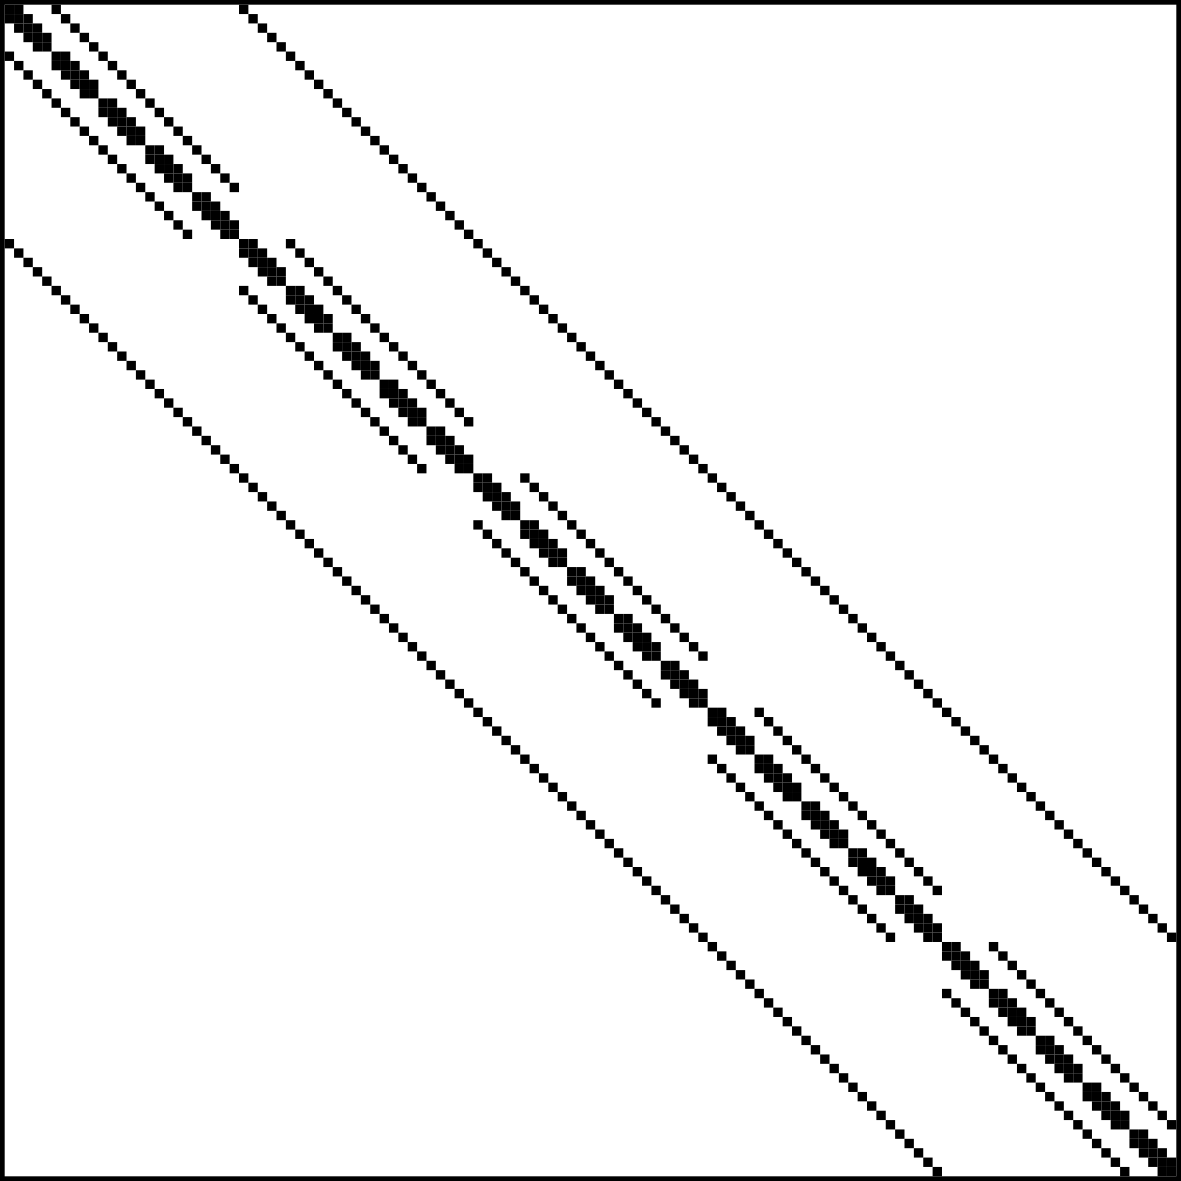
\includegraphics[width=1.0\textwidth]{fig/laplacian_example.png} % second figure itself
        \end{minipage}
        \toccaption{Structured grid and corresponding matrix for a simple Laplacian.}{This example grid with
        an edge size of $d = 5$ is representative of the matric
        matrices used in Section \ref{sec:objsize-fully-structured}}
        \label{fig:laplacian-example-reprint}
    \end{figure}

    The results are displayed in Figure \ref{fig:bytespernnz}. The CSR format's storage requirements are identical for
    both matrix families as they differ only in their nonzero's numerical values. Per nonzero one element is stored in
    the values array and in the column-index array in addition to one entry to the row-pointer array per matrix row. As
    for large matrices the vast majority of rows corresponds to inner nodes which all have $7$ nonzeros, or more
    formally, $\lim \limits_{d\rightarrow \infty} \frac{n_{\text{nnz}}}{n_{\text{row}}} = 7$. The number of rows can
    thus be expressed in terms of the number of nonzeros in the limit $d \rightarrow \infty$ and hence the storage
    requirements per nonzero amount to
    $$
    \lim \limits_{d \rightarrow \infty}\frac{n_{\text{Bytes}}}{n_{\text{nnz}}}
    = \frac{(8 + 4) \cdot n_{\text{nnz}} + 4 \cdot n_{\text{row}}}{n_{\text{nnz}}}
    = 12 + 4\cdot \lim \limits_{d \rightarrow \infty} \frac{n_{\text{nnz}}}{n_{\text{nrow}}}
    = 12 + \frac{4}{7}
    \approx 12.57
    $$

    In order to analyze the relative storage requirements of the corresponding objects in C3SR-format the sizes of the
    individual data arrays must be examined.

    \begin{figure}[H]
      \centering
      \captionsetup{width=0.9\textwidth}
      \begin{tikzpicture}[
        node distance=1cm and 0.1cm,
        vsstyle/.style={draw=gray, minimum height=1cm, minimum width=3cm, fill=dodgerblue4, text=white},
        vstyle/.style={draw=gray, minimum height=1cm, minimum width=3cm},
        pathstyle/.style={->}
      ]
        \node[anchor=west] (DOTS1)
          {$\cdots$};
        \node[vstyle, right=of DOTS1, anchor=west] (VK)
          {$v_{k}$};
        \node[right=of VK, anchor=west] (DOTS2)
          {$\cdots$};
        \node[vstyle, right=of DOTS2, anchor=west] (VKP7)
          {$v_{k+7}$};
        \node[right=of VKP7, anchor=west] (DOTS4)
          {$\cdots$};
        \node[right=of DOTS4, anchor=west] (DOTS5)
          {$\cdots$};
        \node[vstyle, right=of DOTS5, anchor=west] (VKD)
          {$v_{k+7\cdot((d-1) - 2)}$};
        \node[right=of VKD, anchor=west] (DOTS6)
          {$\cdots$};
        \node[anchor=north] (VSDOTS1)
          at ($(DOTS1.south)+(0.5,-1.5)$)
          {$\cdots$};
        \node[vsstyle, right=of VSDOTS1] (VSR)
          {$vs_r$};
        \node[vsstyle, right=of VSR] (VSRP1)
          {$vs_{r+1}$};
        \node[right=of VSRP1] (VSDOTSVSRP1)
          {$\cdots$};
        \node[vsstyle, right=of VSDOTSVSRP1] (VSRPDM2)
          {$vs_{r + ((d-1)-2)}$};
        \node[right=of VSRPDM2] (VSDOTSVSRPDM2)
          {$\cdots$};
        % TODO: RLIE-Triplet (r, k, 7)

        \draw[pathstyle] (VSR.north) |- ($(VSR.north)!0.5!(VK.south)$) -| (VK.south);
        \draw[pathstyle] (VSRP1.north) |- ($(VSRP1.north)!0.5!(VKP7.south)$) -| (VKP7.south);
        \draw[pathstyle] (VSRPDM2.north) |- ($(VSRPDM2.north)!0.5!(VKD.south)$) -| (VKD.south);
      \end{tikzpicture}
      \toccaption{Section within V and VS pertaining to a contiguous segment of inner nodes for matrices from the second
      family.}{Inner nodes yield matrix rows with 7 nonzeros and thus the corresponding section of VS comprises $d-2$
      contiguous elements whose values increase at a constant stride of $7$. This constellation is efficiently condensed
      into a single run-length-increment encoded block.}
    \end{figure}

    \begin{figure}[H]
      \centering
      \captionsetup{width=0.9\textwidth}
      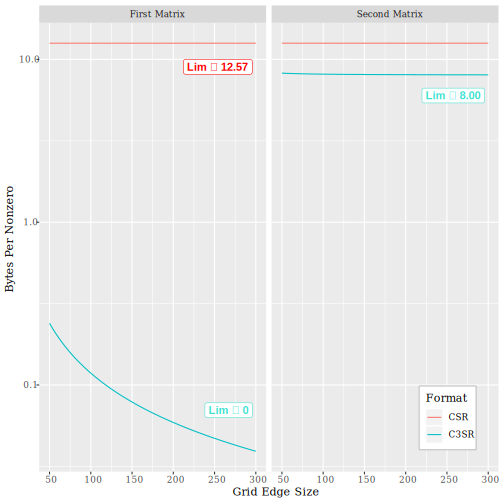
\includegraphics[width=0.9\textwidth]{assets/bytespernnz}
      \toccaption{Object storage size per nonzero matrix element for two families of sparse banded matrices derived from
        fully structured grids for the CSR- and C3SR-formats.}{Analytical convergence limits for $d \rightarrow \infty$
        are annotated next to each curve. The CSR's values are identical for both matrix families and the corresponding
        curve has been annotated only once. The matrix families correspond to the problem exemplified by Figure
        \ref{fig:laplacian-example} and differ only in the values of their nonzero elements, with the first family using
        a single constant value and the second family using unique values for each nonzero. Nonzeros are stored as
        8-byte double precision floats while indices are stored as 4-byte integers. Only values for $d \geq 50$ are
        displayed for the sake of legibility, as the overhead of the C3SR format's compression scheme yields very large
        relative storage size requirements for small matrices.}
      \label{fig:bytespernnz}
    \end{figure}

  \section{Object Size for Perturbed Structured Matrices}

  The matrix-vector multiplication performance of the C3SR format is measured in its CSR-like and vectorized implementations (see \ref{subsec:matrix-vector-multiplication-schemes}). Firstly, a baseline performance is established by comparing the matrix-vector multiplication performance of the C3SR format's CSR-like multiplication scheme introduced in \ref{subsubsec:basic-csr-like-multiplication-scheme} against the CSR format's performance on different sparse banded matrices derived from structured grids and on three different machines. Secondly, the C3SR format's baseline performance is compared against its vectorized counterpart introduced in \ref{subsubsec:vectorized-simd-multiplication-scheme}.

  The following subsection introduces the sparse banded matrices used for the performance benchmarks and their method of acquisition. Subsequently, the results of the performance benchmarks are discussed. Information on the machines used for the benchmarks can be found at the ASC infrastructure wiki\footnote{https://mp-force.ziti.uni-heidelberg.de/kmbeutel/personal-wiki/wikis/ASC-infrastructure} (the KNL was configured to 50\% hybrid mode). All benchmarks were run multi-threaded utilizing the machines' full hardware capabilities.

  \section{Generation of Sparse Banded Matrices as Test Matrices}

    For the purpose of gauging the arithmetic performance, test matrices are created. These matrices resemble the structure of the sparse banded matrices introduced above and are created by iterating through a 3D grid of fixed integral dimensions X, Y, Z and applying a given stencil operation which encodes the desired adjacency relationship of the grid. Nodes requested by the stencil but missing from the grid, i.e. nodes on the grid's outer borders, are omitted, i.e. their corresponding entries in the adjacency matrix carry a zero corresponding to Dirichlet-type boundary conditions.

    The matrix's non-zero entries' numeric values are obtained from evaluating a sinusoidal function at the geometric center point $\vec{r} = (x, y, z)$ inbetween the two nodes in question whereby each Cartesian component $x, y, z$ is scaled by its coordinate's span $X, Y, Z$. An additional offset serves to prevent that entries in the matrix correponding to adjacent nodes according to the stencil incidentally evaluate to 0. The function utilized is $$W(x,y,z; n_x, n_y, n_z) = 2 + \sum \limits_{d \in \{x,y,z\}} \sin{\frac{d}{d_{\text{max}}} \cdot \pi \cdot n_d} $$ where $n_x, n_y, n_z$ are periodicity parameters for each dimensions. The matrix in Figure \ref{fig:laplacian-example} has been created using this method.

    Note that $n_d = 0 \Leftrightarrow \partial_d W(\vec{r}) \equiv 0$, introducing a periodicity in the corresponding dimension $d$. This feature is utilized to control the periodicity in the matrix's values.

    For the purpose of this work two different sets of parameters are utilized generating two different matrices: A smaller matrix generated from a $100 \times 100 \times 100$ grid with the periodicities $n_x = n_y = n_z = 0$ and a second matrix based on the same grid but different periodicities $n_x = 1.1; n_y = 1.2; n_z = 1.3$. Both matrices are generated from a symmetric 7p-stencil operation. The matrices' structures are their grid's equivalent to the example shown in Figure \ref{fig:laplacian-example}.

    The first matrix's values are identical for all rows whose pattern is the same such that \V and \J contain the same small number of elements. The second matrix's rows' values are all unique and thus \V contains approximately $7 \cdot 100^3$ elements (Figure \ref{fig:matrix_stats}).

    \begin{figure}[ht]
      \centering
      \begin{tabular}{ l | c c }
          Array & First Matrix & Second Matrix       \\
        \hline                                       \\
        \V         & $135$          & $6940000$      \\
        \VS        & $1000000$      & $1000000$      \\
        \J         & $135$          & $135$          \\
        \JS        & $1000000$      & $1000000$      \\
        \JP        & $1000000$      & $1000000$      \\
        \RS        & $1000000$      & $1000000$      \\
        Total Size in C3SR format & $\approx 16$MB & $\approx 72$MB \\
        Total Size in CSR Format & $\approx 87$MB & $\approx 87$MB \\
        \hfill
      \end{tabular}
      \caption[Matrices in C3SR format used for matrix-vector multiplication benchmarking.]{\textbf{Matrices in C3SR format used for matrix-vector multiplication benchmarking.} Number of elements is displayed for each array. \V stores double-precision floating-points while all other arrays use 32 bit-wide integers. Additionally, the matrix's size in CSR representation is listed.}
      \label{fig:matrix_stats}
    \end{figure}

    Note that the two matrices share the same structure and thus their only difference is found in \V and \VS. Concerning the vectorized matrix-vector multiplication scheme the first matrix primarily utilizes scheme II (Figure \ref{fig:simd_scheme_diag_collated}) while the second matrix mainly relies on scheme I (Figure \ref{fig:simd_scheme_diag}). The matrices are generated using the asc::matrixgen C++ library\footnote{https://mp-force.ziti.uni-heidelberg.de/asc/AscMatrixGen}.

  \section{Performance of CSR-like Matrix-Vector Multiplication}

    The C3SR format's CSR-like matrix-vector multiplication scheme (referred to as \emph{baseline implementation} hereinafter; see \ref{subsubsec:basic-csr-like-multiplication-scheme}) is compared against its CSR format's pendant using the Eigen C++ library \cite{eigen:website} on three different machines using the sparse banded matrices introduced in the previous section. The results are displayed in Figure \ref{fig:baseline_arithmetic_performance}.

    \begin{figure}[!ht]
      \centering
      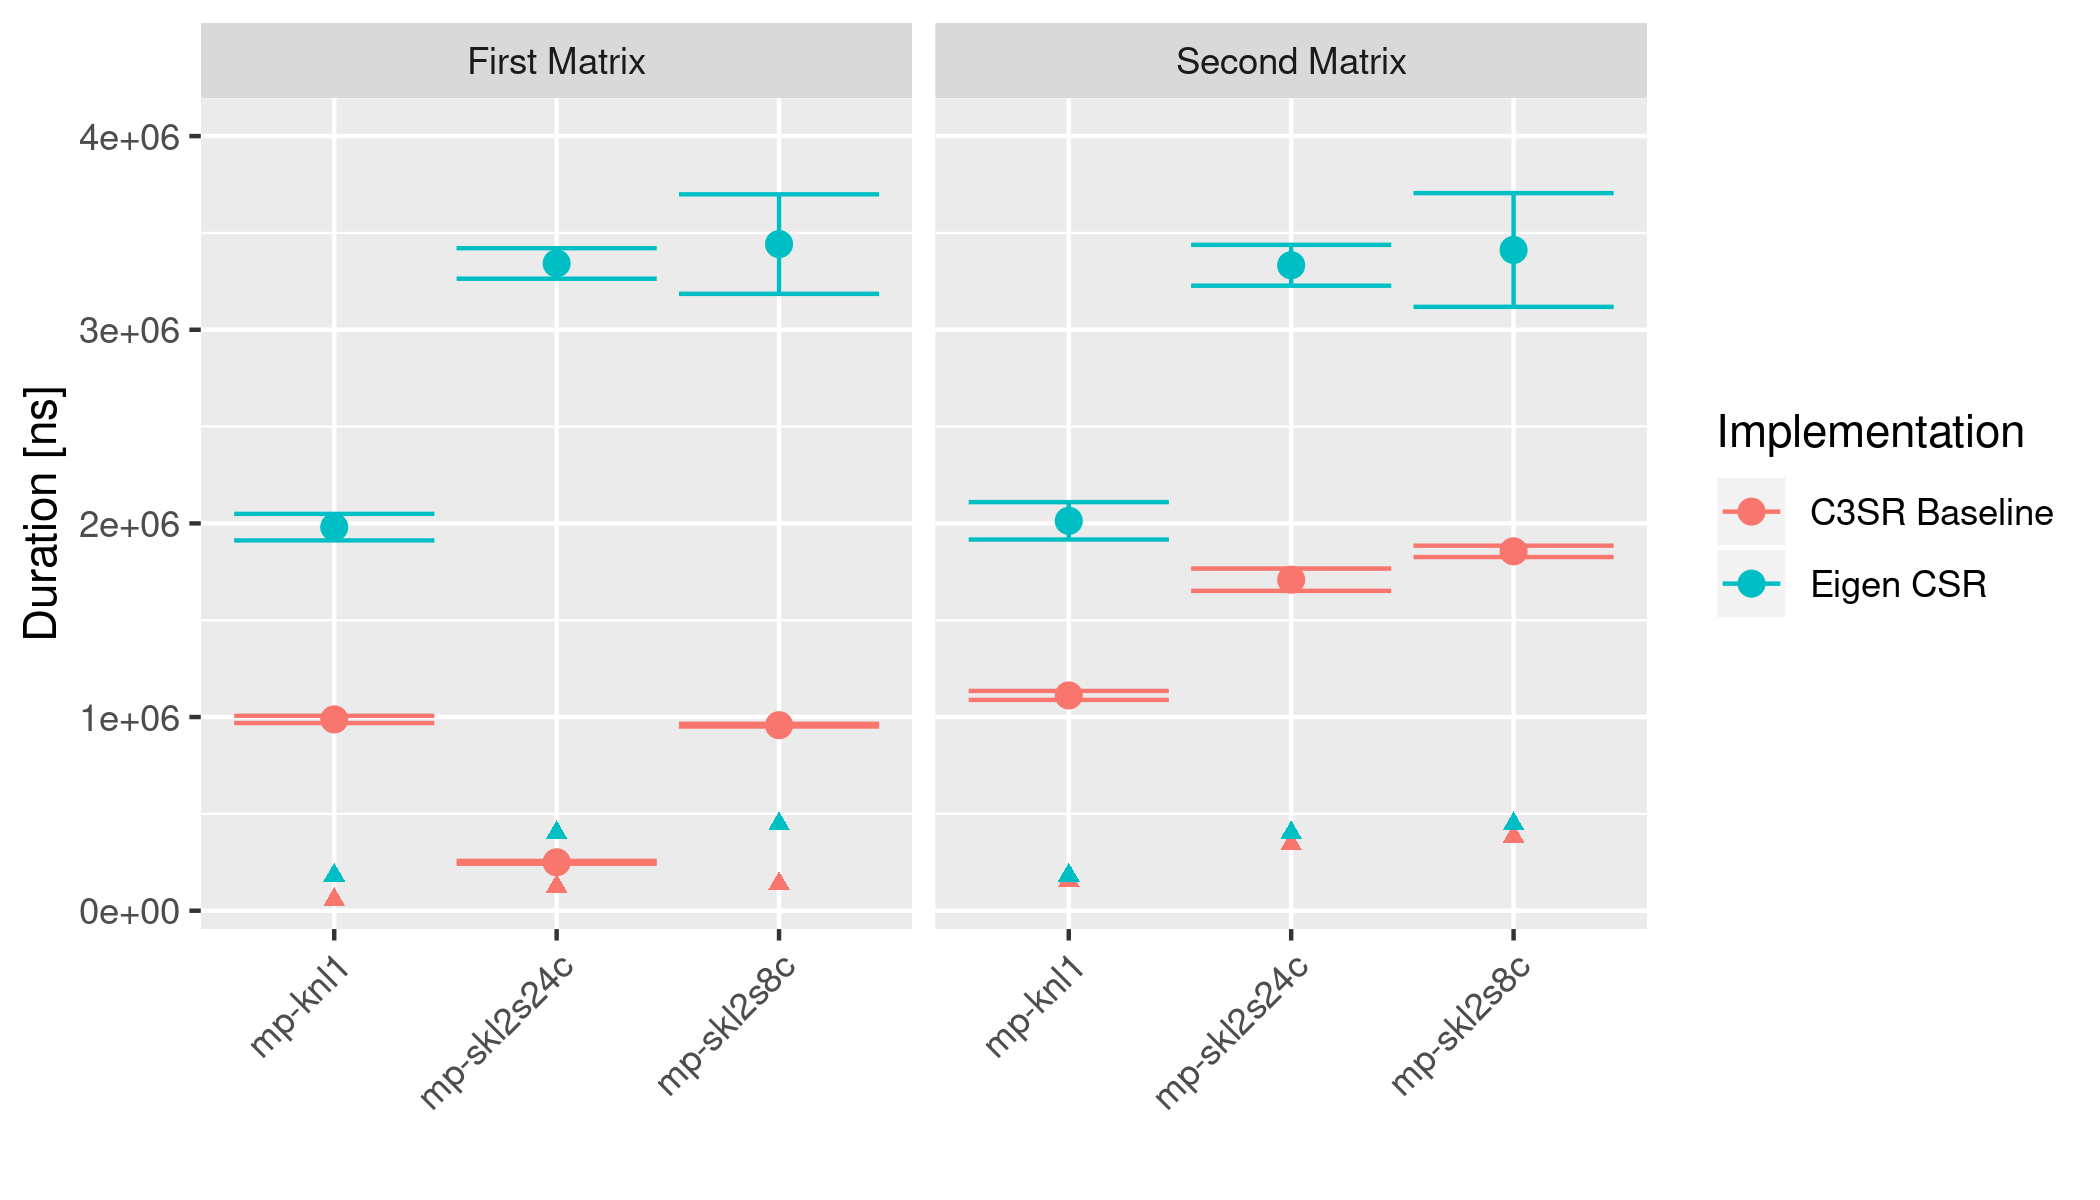
\includegraphics[width=0.9\textwidth]{assets/eigen_vs_c3sr_baseline}
      \caption[Performance comparison of the CSR format against the C3SR format on sparse banded matrices.]{\textbf{Performance comparison of the CSR format against the C3SR format on sparse banded matrices.} The means and sample standard deviations of $10$ samples à $10000$ consecutive matrix-vector multiplications are shown. As the CSR format's representation of the different matrices is identical except for differing numeric values the arithmetic performance is the same save for statistical variance. The triangular symbols denote the theoretical limits as determined by the quotient of the total amount of data involved in a matrix-vector multiplication and the system's theoretical memory bandwidth. Since the matrix storage sizes differ between the storage formats two different limits are displayed.}
      \label{fig:baseline_arithmetic_performance}
    \end{figure}

    By design of the C3SR format, it outperforms the CSR format in the order of magnitude of around $50\%$ irrespective of the machine. This is due to the reduction in the size of the representation of the matrices and the consequent improvement in data locality as the C3SR format's arithmetic is slightly more complex as discussed in \ref{subsubsec:basic-csr-like-multiplication-scheme}. Accordingly, the performance improvement is more pronounced for the first matrix, whose storage size is smaller, entailing speed-up factors of approximately 2, 13, and 3.

    Despite the clear performance benefits the above results have to be qualified further as the implementation of the C3SR format\footnote{https://mp-force.ziti.uni-heidelberg.de/shuell/c3srmatrix} uses a NUMA-aware memory allocation scheme for its data arrays, correctly distributing them across physical memory, suitable for the multi-socket systems utilized for the benchmarks. Conversely, the Eigen C++ library, a general purpose linear algebra and numerics framework, does not tailor its data fields' memory layout in such a way that might lead to performance penalties due to a data distribution inadequate for the access patterns of the multi-threaded arithmetic. Additionally, Eigen internally uses the multi-threading framework OpenMP \cite{openmp:website} which entails a dynamic overhead not present in the implementation of the C3SR format.

  \section{Performance of SIMD Matrix-Vector Multiplication}

    The C3SR format's vectorized multiplication scheme's performance is measured by comparing it against the baseline performance. The implementation of the vectorized multiplication scheme utilizes the explicit SIMD vectorization library UME::SIMD \cite{umesimd2017}. The results are displayed in Figure \ref{fig:arithmetic-performance}.

    \begin{figure}[!ht]
      \centering
      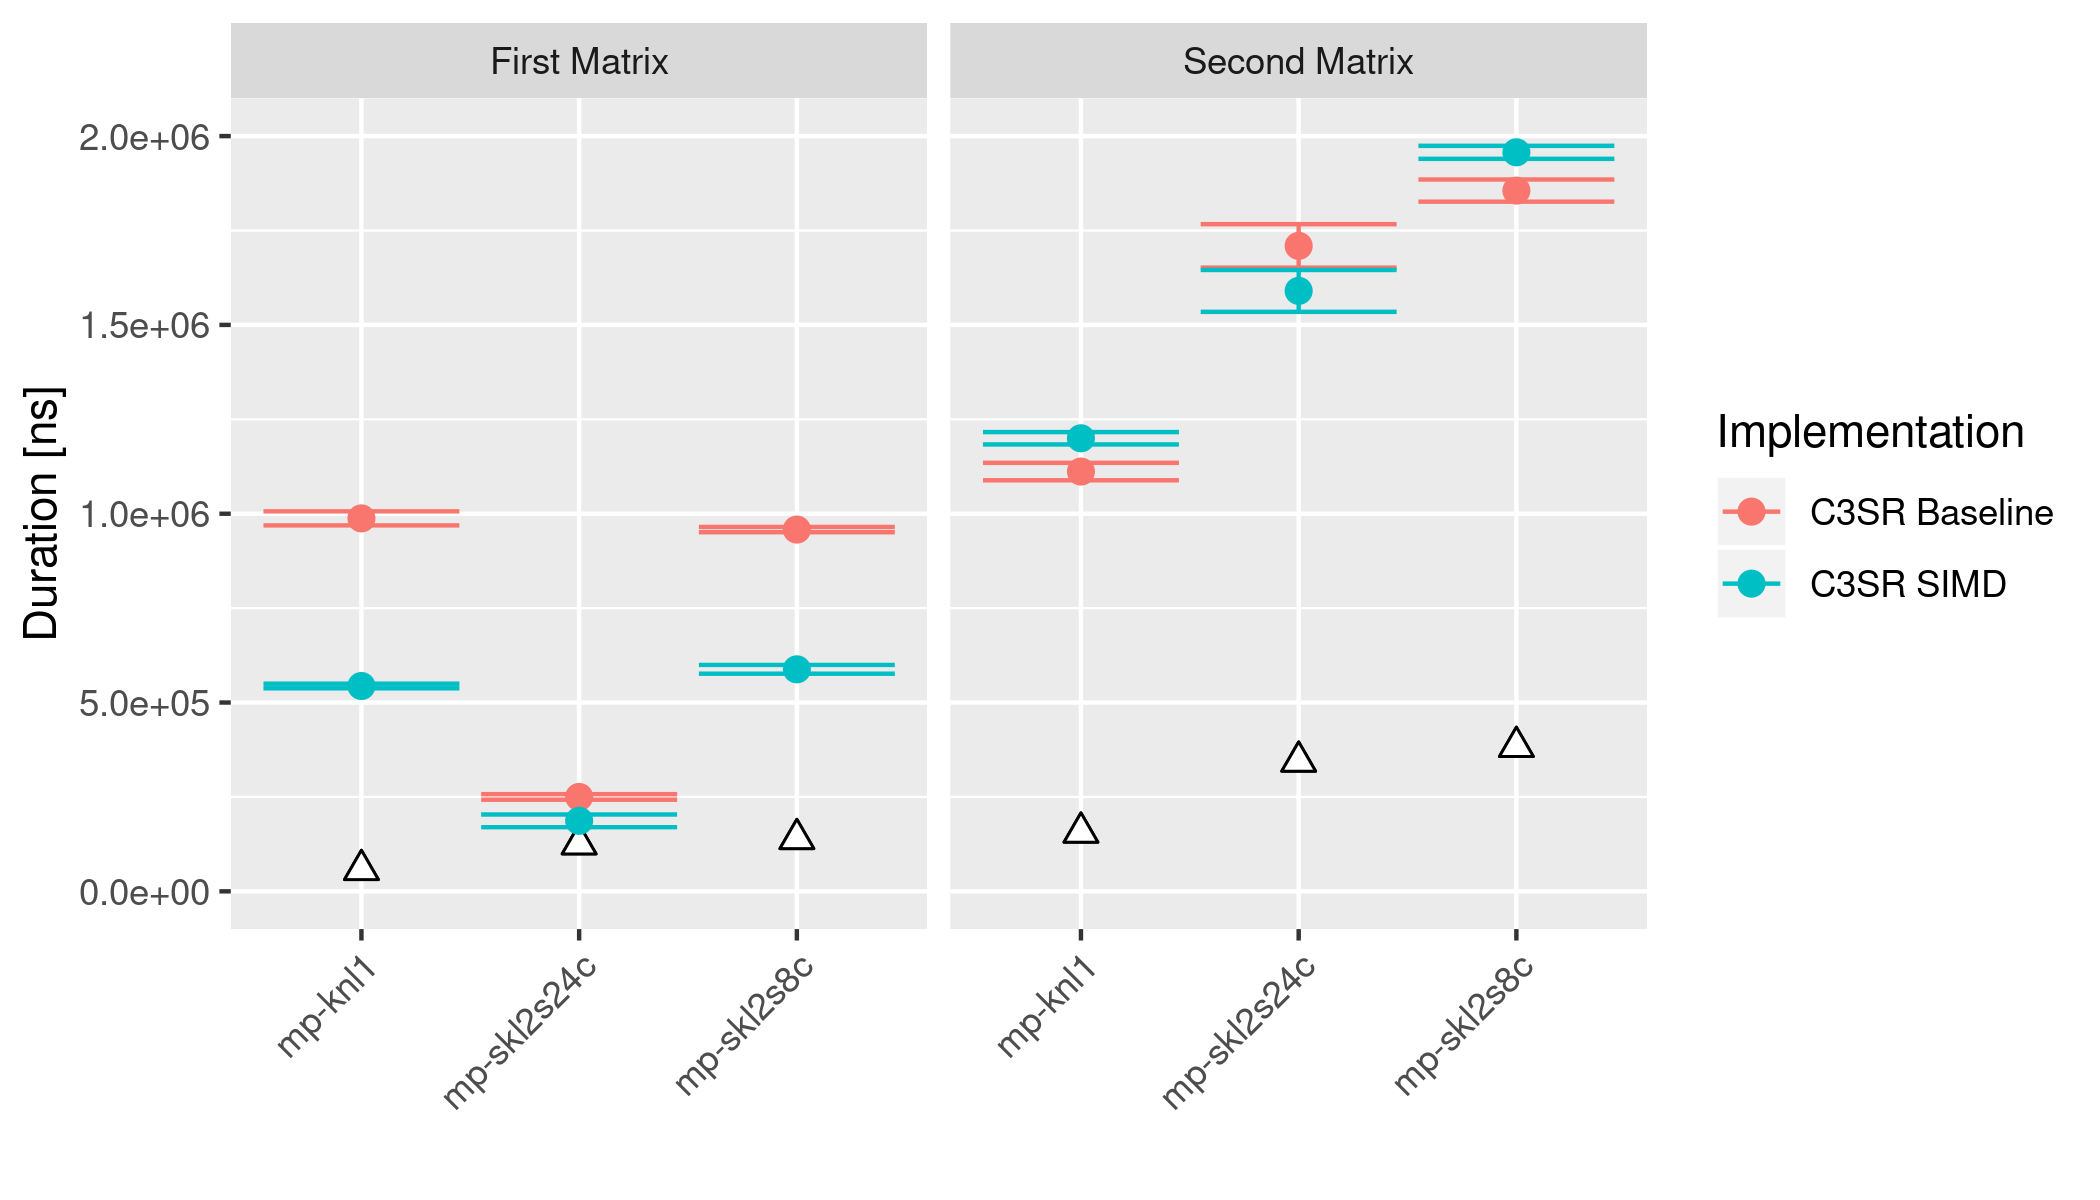
\includegraphics[width=0.9\textwidth]{assets/arithmetic_performance}
      \caption[Performance of C3SR vectorized matrix-vector multiplication scheme compared to baseline implementation.]{\textbf{Performance of C3SR vectorized matrix-vector multiplication scheme compared to baseline implementation.} The means and sample standard deviations of $10$ samples à $10000$ consecutive matrix-vector multiplications are shown. The triangular symbols denote the theoretical limits as determined by the quotient of the total amount of data involved in a matrix-vector multiplication and the system's theoretical memory bandwidth.}
      \label{fig:arithmetic-performance}
    \end{figure}

    Sparse matrix-vector multiplication is a memory-bound computation so that the efficacy of a vectorized arithmetic implementation depends very strongly on the amount of data that is required to be read from memory and whether the dynamic overhead involved in determining the applicable SIMD scheme is compensated by a speed-up in arithmetic. This fact is reflected in the measurements as for the second matrix the SIMD implementation is generally slower than the baseline implementation. Only for the first matrix a significant speed-up can be observed on every machine. However, this might be partly due to the fact that the second matrix's SIMD multiplication scheme is less performant as it involves strided loads from memory which might equate to regular gather operations on the hardware used for this benchmark (see \ref{subsubsec:vectorized-simd-multiplication-scheme}).

  \section{Further Considerations}

    By evidence of the performance benchmarks presented in the previous section the basis for the performance gain in the arithmetic of the C3SR format with respect to the CSR format for sparse banded matrices is the reduction of the matrix's total storage size in memory leading to big improvements in data locality during matrix-vector multiplication.

    The C3SR format's storage scheme is tailored to minimize the matrix' storage size in memory. However, depending on how the matrix object is created in memory, adhering to the storage scheme to its full extent may not be optimal as it might limit parallelism during object construction. The data arrays' contents are strongly coupled such that the workload cannot be trivially spread across multiple threads. Instead, it might be advisable to partition the matrix into equally sized slices whose independent C3SR objects can be created in parallel. Finally, these distinct C3SR objects corresponding to the matrix slices are then transformed into a singular object by concatenating the data arrays requiring that the index-pointer arrays are offset by the number of rows preceding their first matrix row.

    \begin{figure}[ht]
      \centering
      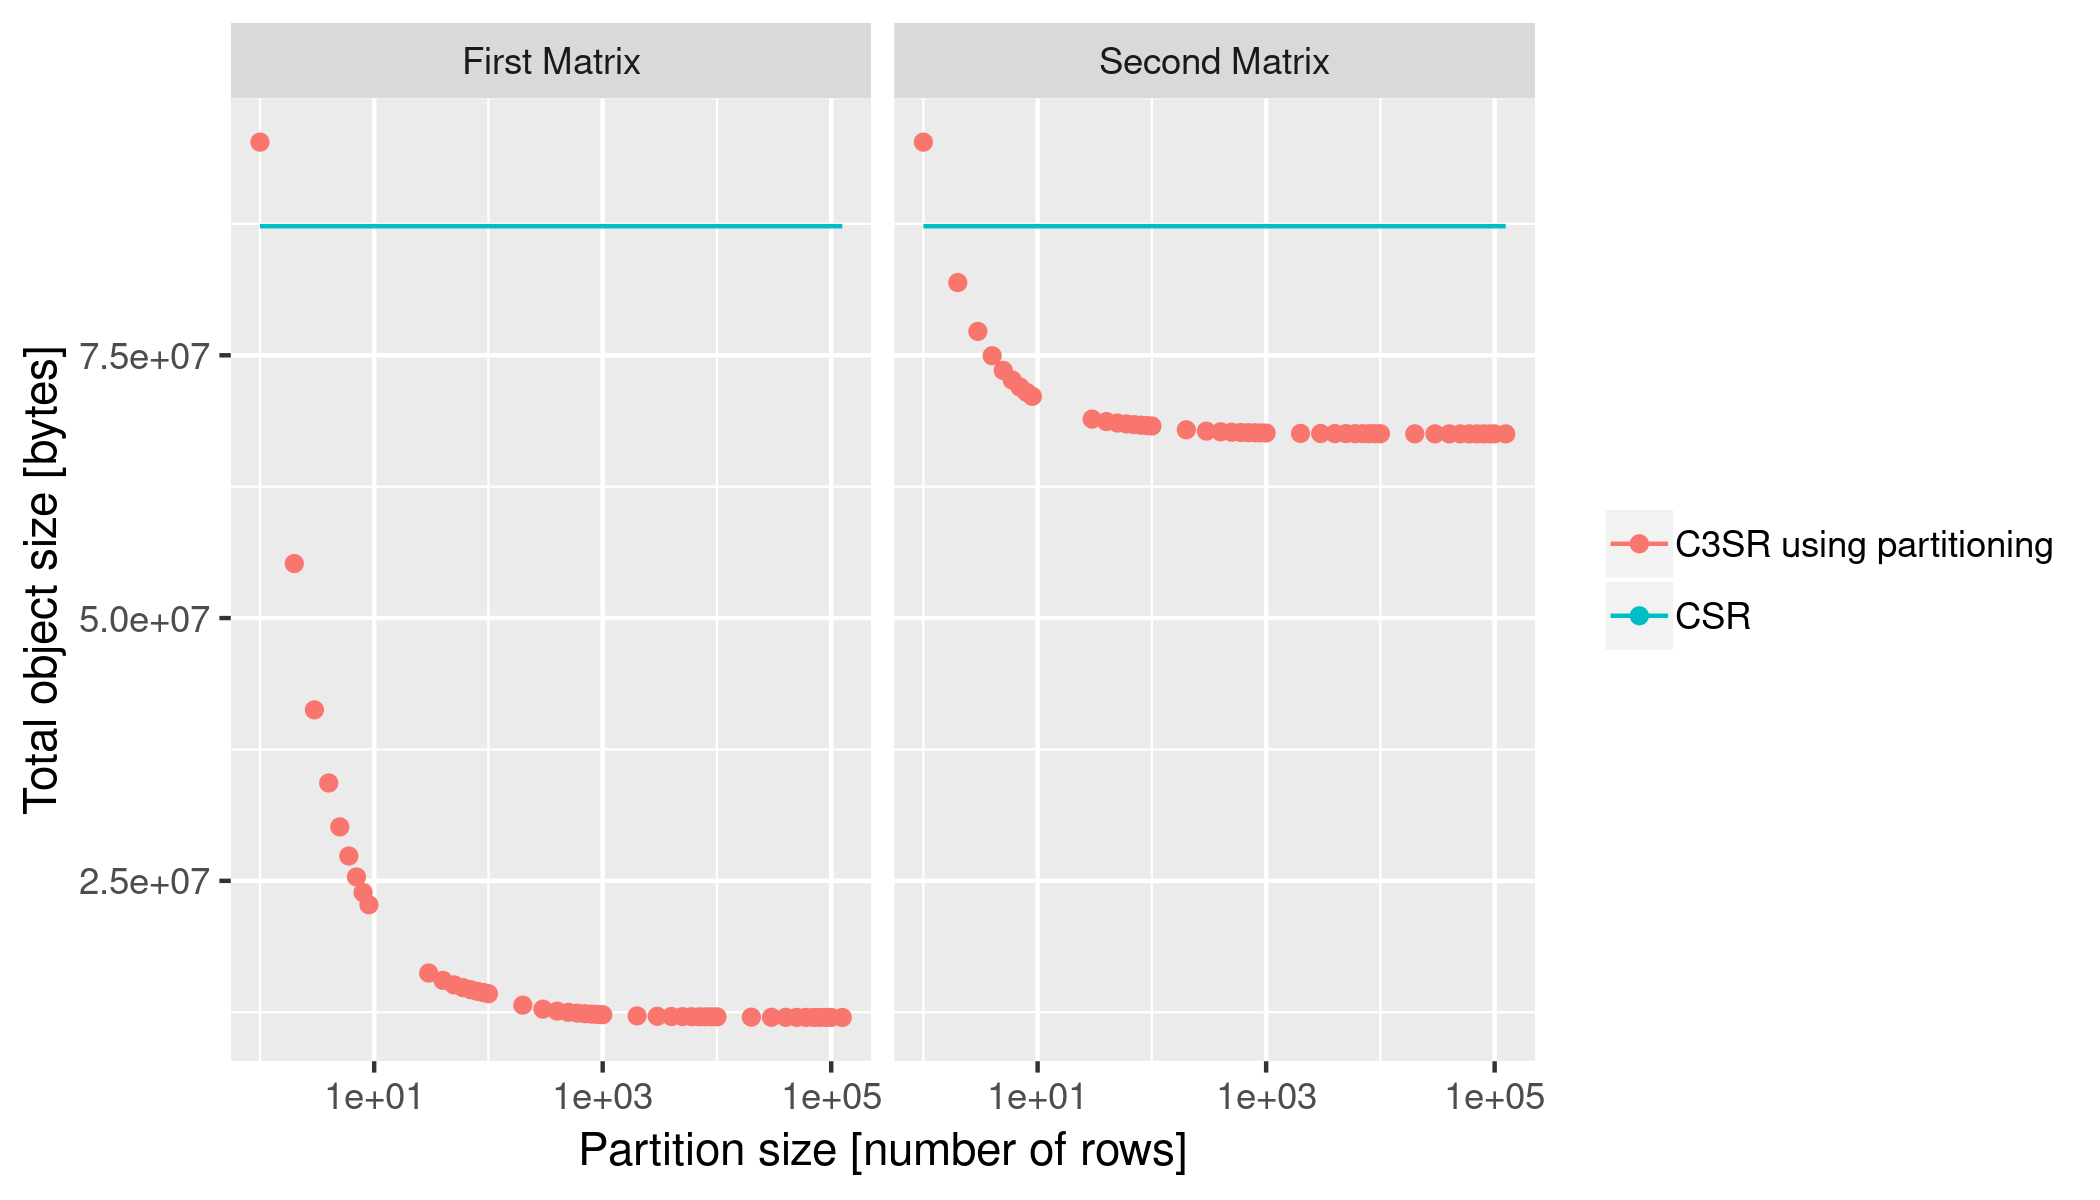
\includegraphics[width=0.9\textwidth]{assets/structured_grid_matrix_heap_size}
      \caption[C3SR matrix storage size depending on partition size.]{\textbf{C3SR matrix storage size depending on partition size.} Numeric values are stored using double precision floating-point numbers while all other arrays utilize 32 bit integers. A point of diminishing returns is reached at a partition size of around 1000, past which the storage size in memory does not shrink significantly. Thus, creating C3SR objects using partition sizes of 1000 and larger may yield a similar performance while speeding up the creation of the object. For comparison the corresponding CSR format's storage size is provided.}
      \label{fig:structured_grid_matrix_heap_size}
    \end{figure}

    In order to establish an estimate for an apt partition size Figure \ref{fig:structured_grid_matrix_heap_size} displays the total storage size depending on the partition size for the two matrices used for the performance benchmarks. It is evident that there exists a point of diminishing returns past whose partition size there is no significant gain in storage size reduction. This point is reached when the sizes of \V and \J, the two arrays responsible for the reduction in storage size for the C3SR format, fall significantly below the fixed sizes of the remaining arrays, which constitute a minimum to the storage size.

    Thus, the performance benefits of the C3SR format may be kept even when trading larger storage sizes in favor of the parallelizability of the application.


    \chapter{Outlook}

Scan of row-sizes for load-balancing mvm.

Further shrink COMP by including it indirectly into JS. COMP analysis is much faster on the RLI-enc'd arrays.

Further control over NUMA allocation. Mapping of arrays' sections to NUMA nodes can only be done perfectly AFTER the
object has been created and it known, which NUMA nodes access which sections of V (complex matrices).

\Todo{SIMD kann nicht sinnvoll genutzt werden, höchstens für kleine Objekte. Skalar MVM genauso schnell}

\Todo{Proper NUMA control - Tbb does not allow for it}

%% Stuff from SRP

  This report introduces the threefold compressed sparse row matrix storage format (C3SR) which has been designed to
  adapt the CSR format to improve the performance of matrix-vector multiplication for sparse banded matrices derived
  from structured grids. Significant performance benefits have been demonstrated for two different sparse banded
  matrices based on a $100 \times 100 \times 100$ grid utilizing the basic CSR-like matrix-vector multiplication scheme
  of the C3SR format.

  A vectorized arithmetic scheme could only be shown to provide performance improvements for the matrix whose storage
  size in memory is significantly smaller implying that the matrix-vector multiplication is bound by the system's memory
  bandwidth. Thus, for the machines utilized for this work, the applicability of vectorization for the arithmetic
  depends strongly on the sparse banded matrix in question. For some systems, it showed worse performance than the
  baseline CSR-like implementation.

  \section*{Future Work}

    In order to gauge arithmetic performance, this project uses few synthetic matrices which, albeit being realistic
    examples, cover only very little of the total spectrum of sparse banded matrices that occur in real-life
    applications. Especially heterogeneous domains as discussed in section \ref{subsec:structured-grid-matrices} yield
    sparse matrices which are only partially structured. These scenarios have to be investigated separately in terms of
    arithmetic performance.


%  \part{matrixgen - A Sparse Matrix Creation Toolkit}
%
%    During the creation of the part 1 experimentation with many matrices of various shapes and sizes was required. For this
the source code grew and eventually was encapsulated into an independent project.

Focus on grids derived from structured grids; but also many simple tools

Idea: Preset matrices for all purposes.

As this was an aid to development of caesr the focus lies on simple interface, and consistency. Where necessary ease of
use and maintability were preferred over performance gain.

Note: Makes intensive use of TMP the capabilities of which have enjoyed massive improvements over the last iterations of
the c++ standard. hence C++20 is used and users with version limitations (such as cuda zealots) are required to write a
simple wrapper to create a static library.

blablbal ... Output object format specified as template parameter making the interface easily expandable to different
output formats.

%    \chapter{Available Modules}

  \section{\texttt{matrixgen::create}}

    \begin{lstlisting}[language=C++, caption={Basic usage of `matrixgen::create'}]
      #include <iostream>
      #include <matrixgen/core>
      int main() {

        // Choose the matrix object type to return.
        using Matrix_t = Eigen::Matrix<double, Eigen::Dynamic, Eigen::Dynamic>;

        // Create the object by specifying the matrix's dimensions and its values.
        auto matrix = matrixgen::create<Matrix_t>(3, 4,
            {3.1, 0.0, 0.0, 5.2,
             1.0, 0.0, 1.0, 0.0,
             1.0, 7.7, 0.0, 0.0});

        // Use the object.
        std::cout << matrix << std::endl;
        return 0;
      }
    \end{lstlisting}

    % CONTINUEHERE: Output of the above code.


  \printbibliography
  \addcontentsline{toc}{chapter}{\bibname}

  % Avowal

  \newpage

\begin{tikzpicture}[
  remember picture,
  overlay,
  every node/.style={inner sep=0, outer sep=0}
    ]
  \node[anchor=north,
        font=\large,
        align=left,
        text width=16cm] (TEXT)
    at ($(current page.north west)+(0.5\paperwidth, -5)$)
    {\Huge{Erklärung}\large\\\vspace{2cm}
     Ich versichere hiermit, dass ich diese Arbeit selbstständig verfasst habe und keine anderen als die angegebenen
     Quellen und Hilfsmittel verwendet habe.};
  \node[anchor=north west, font=\large]
    at ($(TEXT.south west)+(0, -1)$) (DATEDECL)
    {Heidelberg, den \hspace{5cm} Unterschrift:};
  \draw (DATEDECL.south east) -- ($(DATEDECL.south east)+(5, 0)$);

\end{tikzpicture}

\newpage


\end{document}
